\documentclass {report}
\addtolength{\textwidth}{2 cm}
\addtolength{\textheight}{3 cm}
%\usepackage[latin1]{inputenc}
\usepackage[utf8]{inputenc}
\usepackage{textcomp}
\usepackage{amsmath,amssymb,amsfonts,mathrsfs}
\usepackage{bm}
\usepackage{color, xcolor,epic,eepic,multicol,graphicx}
\usepackage[T1]{fontenc}
\usepackage{pstricks, pstricks-add}
\usepackage[all]{xy}
\usepackage[french]{babel}
\usepackage{ulem, listings, ccaption}
\usepackage[framed,amsmath,thmmarks]{ntheorem}
\usepackage{pgfgantt}
\usepackage{animate}
\theoremheaderfont{\upshape \bfseries}
\theoremseparator{:} 

\newcommand{\prodscal}[2]{\left\langle#1,#2\right\rangle}
\newcommand{\gs}[1]{\textbf{\underline{#1}}}

\newtheorem{defi}{Définition}[section]
\newcommand{\defin}[1]{\begin{defi}#1\end{defi}\vspace{0.3cm}}
\newcommand{\defibox}[1]{\hspace{-0.7cm}\fbox{\begin{minipage}{14cm}\begin{defi}#1\end{defi}\end{minipage}}\vspace{0.3cm}}
\renewcommand{\thedefi}{\empty{}} 

\newtheorem{defis}{Définitions}[section]
\newcommand{\defins}[1]{\begin{defis}#1\end{defis}\vspace{0.3cm}}
\newcommand{\defisbox}[1]{\hspace{-0.7cm}\fbox{\begin{minipage}{14cm}\begin{defis}
#1\end{defis}\end{minipage}}\vspace{0.3cm}}
\renewcommand{\thedefis}{\empty{}} 

\newtheorem{theo}{Théorème}[section]
\newcommand{\theor}[1]{\begin{theo}#1\end{theo}\vspace{0.3cm}}
\newcommand{\theobox}[1]{\hspace{-0.7cm}\fbox{\begin{minipage}{14cm}\begin{theo}
#1\end{theo}\end{minipage}}\vspace{0.3cm}}

\newtheorem{propr}[theo]{Propriété}
\newcommand{\propri}[1]{\begin{propr}#1\end{propr}\vspace{0.3cm}}
\newcommand{\proprbox}[1]{\hspace{-0.7cm}\fbox{\begin{minipage}{14cm}\begin{propr}
#1\end{propr}\end{minipage}}\vspace{0.3cm}}

\newtheorem{proprs}[theo]{Propriétés}
\newcommand{\propris}[1]{\begin{proprs}#1\end{proprs}\vspace{0.3cm}}
\newcommand{\proprsbox}[1]{\hspace{-0.7cm}\fbox{\begin{minipage}{14cm}\begin{proprs}
#1\end{proprs}\end{minipage}}\vspace{0.3cm}}

\newtheorem{propo}[theo]{Proposition}
\newcommand{\propos}[1]{\begin{propo}#1\end{propo}\vspace{0.3cm}}
\newcommand{\propobox}[1]{\hspace{-0.7cm}\fbox{\begin{minipage}{14cm}\begin{propo}
#1\end{propo}\end{minipage}}\vspace{0.3cm}}

\newtheorem{lemm}[theo]{Lemme}
\newcommand{\lemme}[1]{\begin{lemm}#1\end{lemm}\vspace{0.3cm}}
\newcommand{\lemmbox}[1]{\hspace{-0.7cm}\fbox{\begin{minipage}{14cm}\begin{lemm}
#1\end{lemm}\end{minipage}}\vspace{0.3cm}} 

\newtheorem{corr}[theo]{Corollaire}
\newcommand{\corro}[1]{\begin{corr}#1\end{corr}\vspace{0.3cm}}
\newcommand{\corrbox}[1]{\hspace{-0.7cm}\fbox{\begin{minipage}{14cm}\begin{corr}
#1\end{corr}\end{minipage}}\vspace{0.3cm}}
\everymath{\displaystyle}
\newtheorem{affi}{Affirmation}
\newtheorem{rema}{Remarque}

\newrgbcolor{fftttt}{1 0.2 0.2}
\newrgbcolor{ttffqq}{0.2 1 0}
\psset{xunit=9.62cm,yunit=2.27cm,algebraic=true,dotstyle=o,dotsize=3pt 0,linewidth=0.8pt,arrowsize=3pt 2,arrowinset=0.25}
\renewcommand{\contentsname}{Sommaire}
%\setlength{\unitlength}{1cm}
\graphicspath{Images_Fichiers}
\setlength{\parskip}{.3cm}
\everymath{\displaystyle}
\definecolor{string}{rgb}{0.317,0.49,0.345}
%\definecolor{keyword}{rgb}{0.80,0.47,0.2}
%\definecolor{comments1}{rgb}{0,0.6,0}
\definecolor{comments2}{rgb}{0.37,0.55,0.32}
%\definecolor{fonctions}{rgb}{0,0.6,0}
\definecolor{attributs}{rgb}{0.59,0.43,0.56}
\lstset{		language=Java,
 				backgroundcolor=\color{black},
                basicstyle=\color{white}\small,
                keywordstyle=\color{orange}\ttfamily,
                stringstyle=\color{olive}\ttfamily,
                commentstyle=\color{gray}\ttfamily,
                morecomment=[s][\color{lime}]{/**}{**/},
                keepspaces=true,
                morekeywords={module, export, constructor, let, of, number}, 
                showstringspaces=false, 
                tabsize = 2,
                morekeywords={[2]taille, choix, nbIterations, geo, position, links, to, hashNumber, x, y, z}, 
                keywordstyle={[2]\color{attributs}},
                morekeywords={[3]go, goForTheFirstTime, getValue, allKeys, putValue, tan, angleBetweenTwoVectorsBetween0andPi, newFrom, substract, min, max, add, scale, push, setPosition },
                keywordstyle={[3]\color{yellow}}, 
                morekeywords={[4]0, 1, 2, 3, 4, 5, 6, 7, 8, "9"}, 
                keywordstyle={[4]\color{blue}}
}
\newcommand{\Z}{\mathbb{Z}}
\newcommand{\R}{\mathbb{R}}
\newcommand{\Q}{\mathbb{Q}}
\newcommand{\N}{\mathbb{N}}
\newcommand{\D}{\mathbb{D}}
\newcommand{\C}{\mathbb{C}}
\begin{document}
\baselineskip=0.5cm
\huge{GRAFF Jonathan}
\vspace{5cm}
\begin{center}
\Huge{\bf Stage : \\ \  \\Les Surfaces minimales}
\end{center}
\vspace{6cm}
\hspace{2cm} \huge{Sous la direction de M. Vincent Vigon}
\vspace{2cm}\\
\hspace*{10.5cm}\Large{Master 1 CSMI \vspace{1cm}\\ \hspace*{5cm}Année universitaire 2016-2017 - Semestre 2}\normalsize
\tableofcontents
\newpage

\chapter[Introduction]{\uline{Introduction}}

Ce stage de master 1 a porté sur les surfaces minimales. Dans un premier temps, j'ai tout d'abord lu de la théorie pour comprendre ce qu'était une surface minimale, aussi bien intuitivement que formellement. \\

Les surfaces minimales ont de nombreuses applications, notamment en physique et en mécanique. Les surfaces prises par des bulles de savon sont toujours minimales, le film savonneux tendant toujours à prendre une forme qui minimise son aire : 

\begin{figure}[h!]
   \begin{minipage}[b]{0.5\linewidth}
      \centering 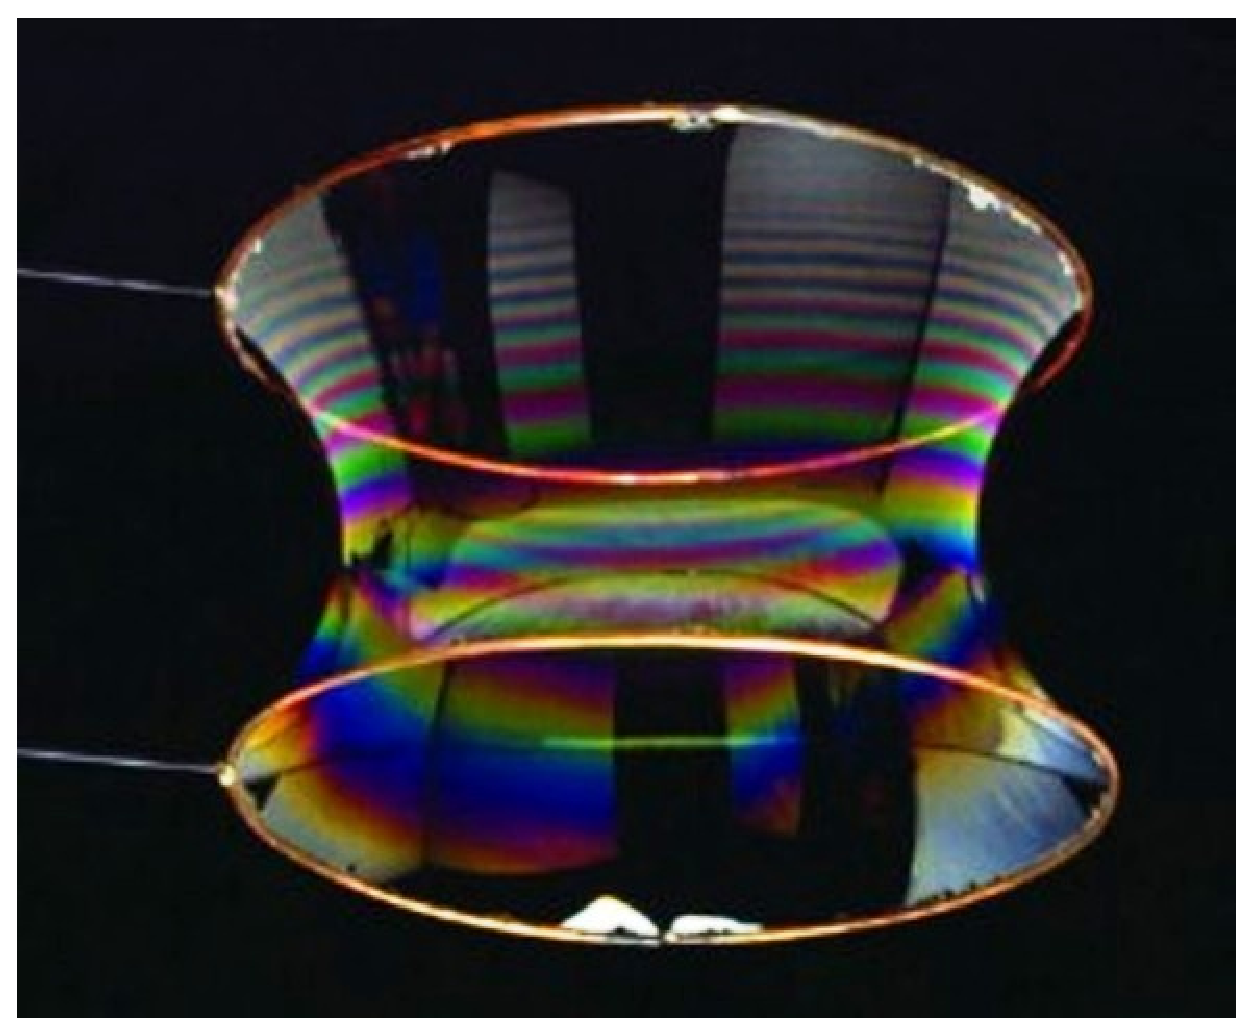
\includegraphics[scale=0.25]{Images_Fichiers/savoncaten.eps}
      \legend{Un caténoïde}
   \end{minipage}
   \begin{minipage}[b]{0.5\linewidth}   
     \centering 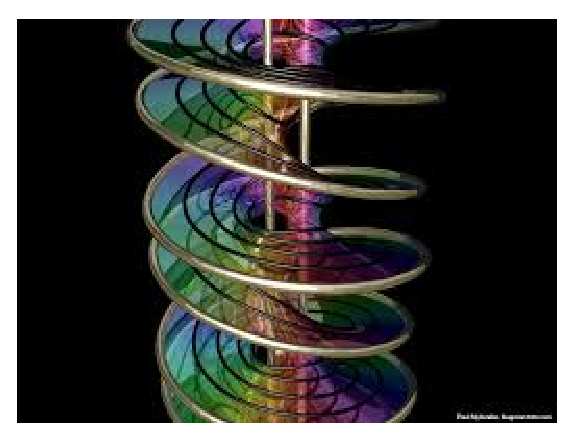
\includegraphics[scale=0.6]{Images_Fichiers/savonhelico.eps}
      \legend{Un hélicoïde}
   \end{minipage}
\end{figure}

\begin{figure}[h!]
   \begin{minipage}[b]{0.40\linewidth}
      \centering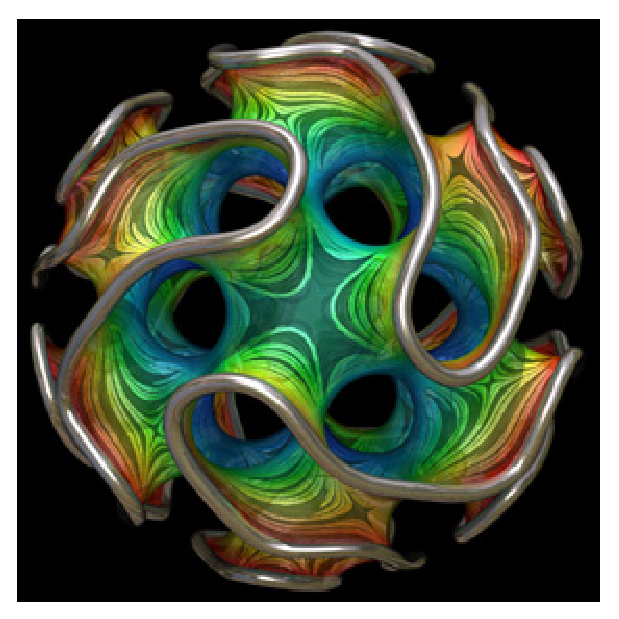
\includegraphics[scale=0.4]{Images_Fichiers/savongyroid.eps}
      \legend{Une gyroïde}
   \end{minipage}
   \begin{minipage}[b]{0.3\linewidth}   
     \centering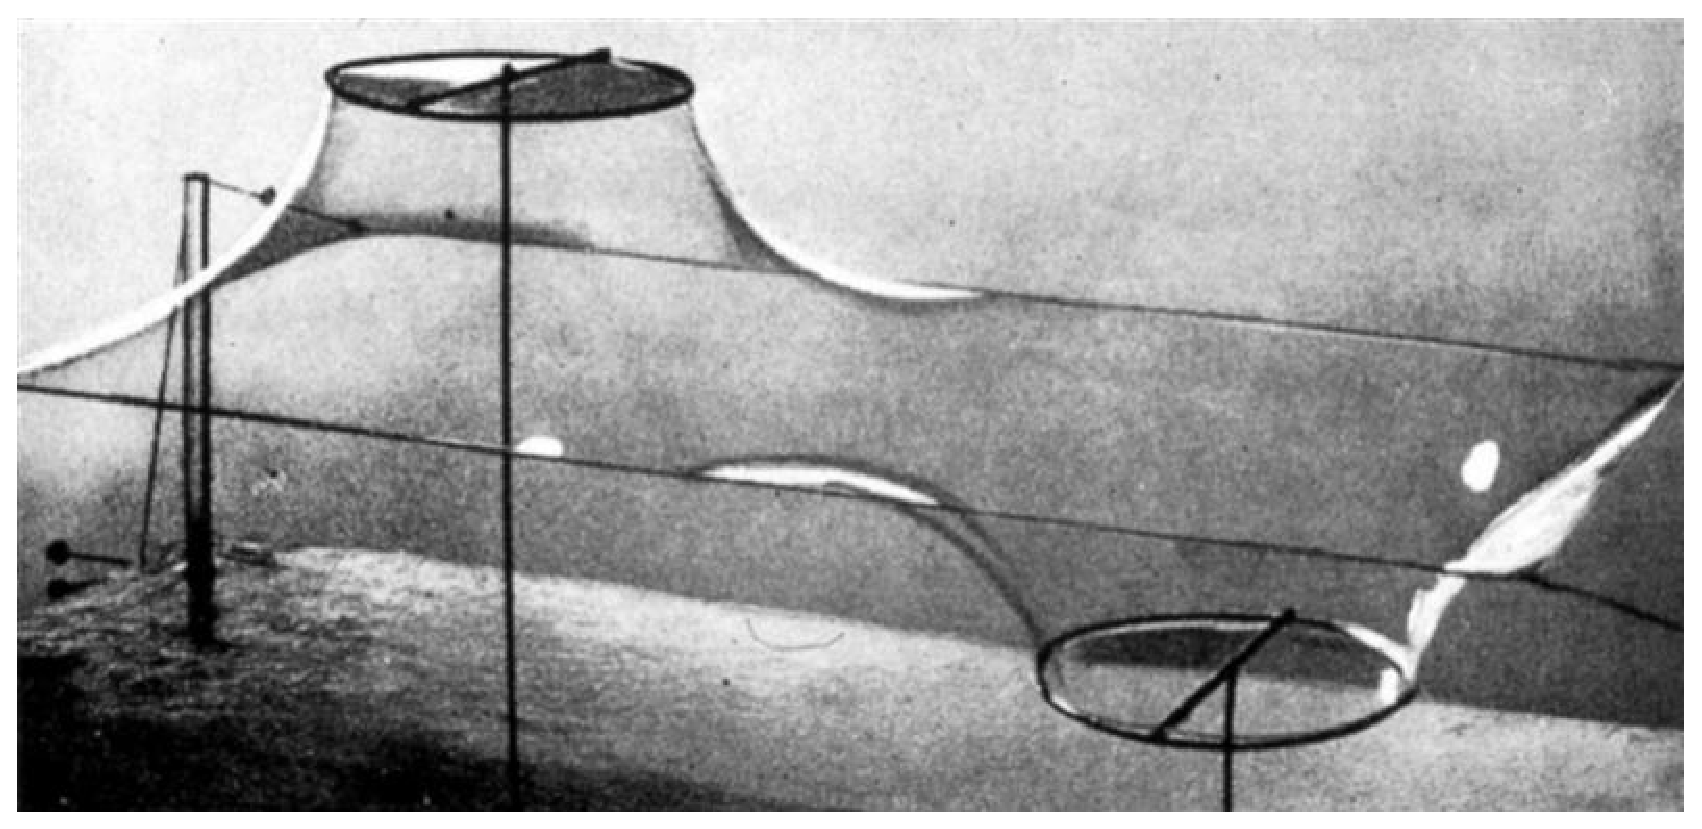
\includegraphics[scale=0.3]{Images_Fichiers/savonriemann.eps}
      \legend{Une surface de Riemann}
   \end{minipage}
\end{figure}
\newpage

Dans le domaine artistique, plusieurs artistes ont également sculpté des surfaces minimales, et le stade olympique de Munich a un toit dont sa surface est minimale : 

\begin{figure}[h!]
   \begin{minipage}[b]{0.45\linewidth}
      \centering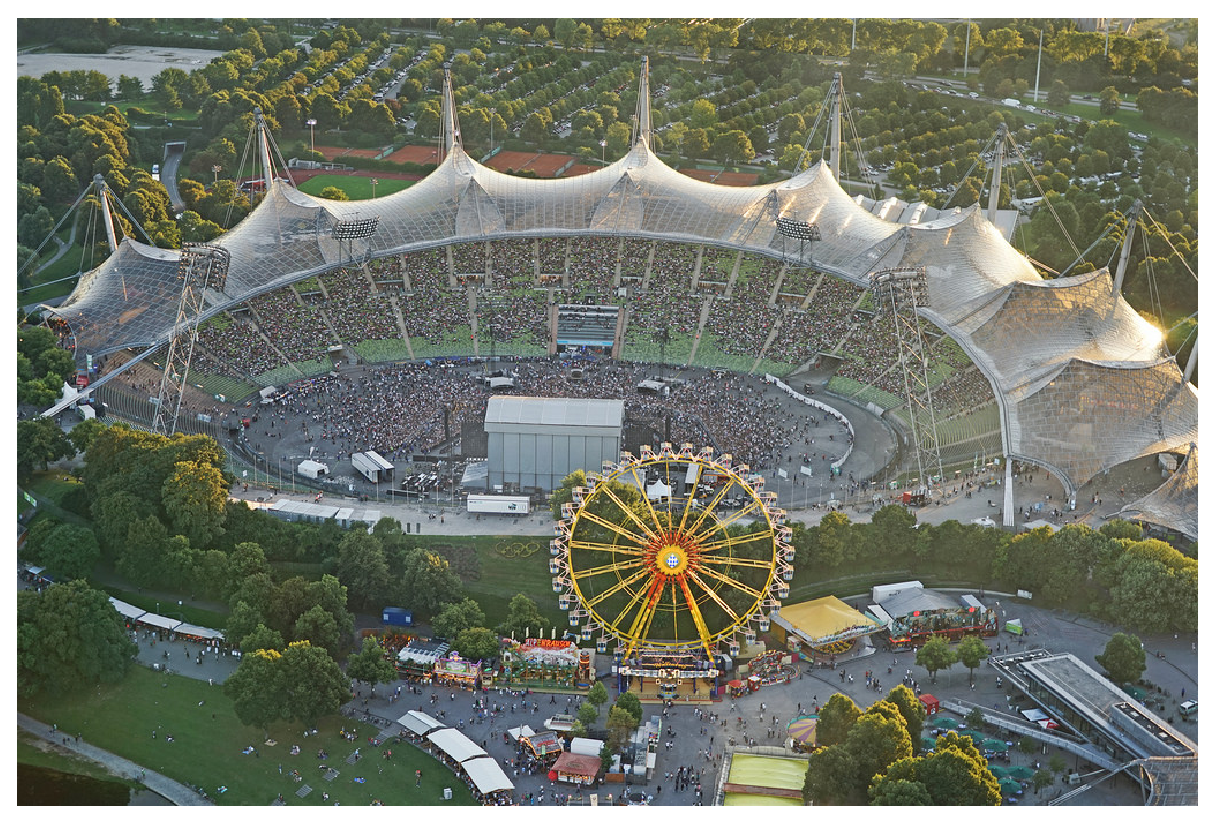
\includegraphics[scale=0.3]{Images_Fichiers/stade1.eps}
   \end{minipage}
    \begin{minipage}[b]{0.50\linewidth}   
     \centering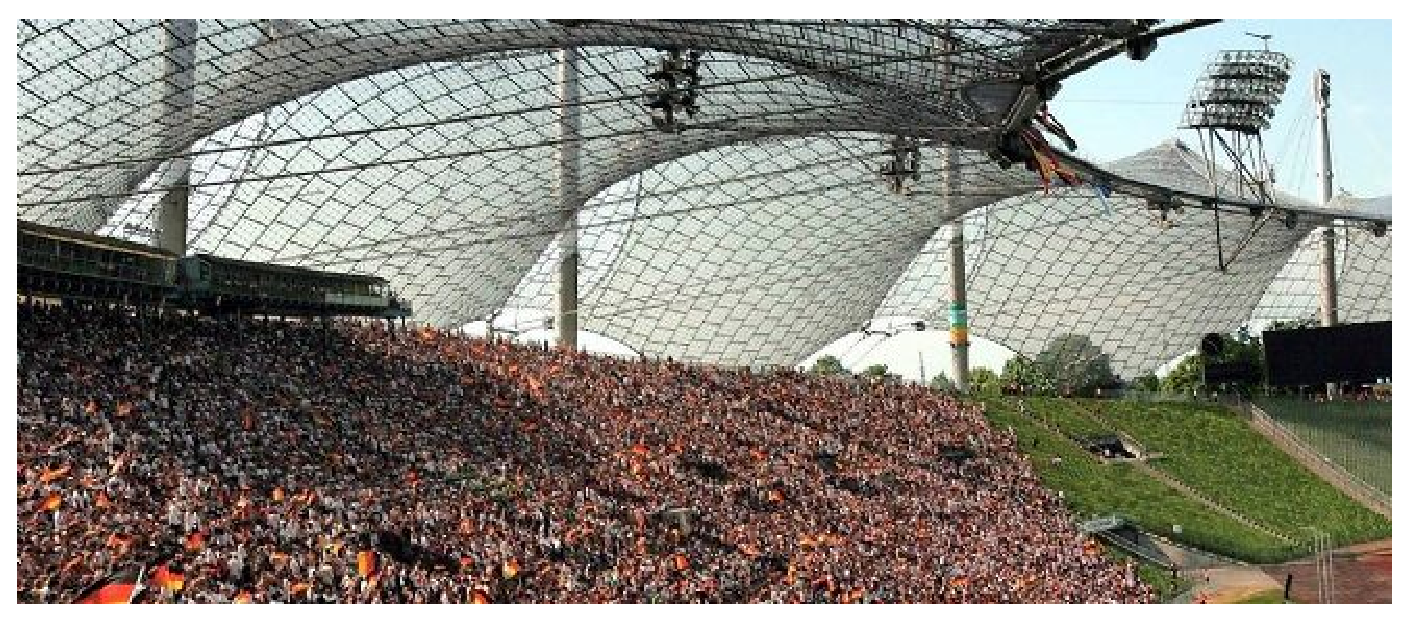
\includegraphics[scale=0.35]{Images_Fichiers/stade2.eps}
   \end{minipage}
\end{figure}

Il y a deux façons de comprendre la notion de surface minimale, soit comme une surface de courbure moyenne nulle, soit comme une surface d'aire localement minimale. Nous détaillerons et verrons quelques liens entre ces deux concepts.

Ensuite, j'ai programmé en Typescript un algorithme pour pouvoir répondre au problème de Plateau, à savoir comment trouver une surface minimale, étant donné ses bords. L'algorithme, ainsi que les résultats obtenus sous Mathis seront détaillés dans cette partie.

Enfin, j'ai implémenté une formule dûe à Weierstrass, qui permet, pour deux fonctions complexes données, de créer une surface minimale. Toute surface minimale peut être exprimée sous cette forme, donc en théorie, nous pouvons tracer n'importe quelle surface minimale à partir de cet algorithme. 

\chapter[Théorie sur les surfaces minimales]{\uline{Théorie sur les surfaces minimales}}

\section[Surfaces]{\uline{Surfaces}}

\subsection[Définition]{\uline{Définition}}

\defisbox{\ \\
\begin{itemize}
\item Soit $\mathscr{U}$ une partie de $\R^2$. On dit qu'une application $x: \mathscr{U} \rightarrow \R^3$ est un \uline{patch} (ou une surface locale) si $x$ est différentiable sur $\mathscr{U}$.
\item Un patch est dit régulier si pour tout $(u,v)$ de $\mathscr{U}$, la matrice jacobienne $\mathscr{J}_x(u,v)$ est de rang 2.
\item Un ensemble $\mathscr{M}$ de $\R^3$ est une surface régulière si pour tout point $p$ de $\mathscr{M}$, il existe un ouvert $\mathscr{U}$ de $\R^2$, un voisinage $\mathscr{V}$ de $p$ dans $\mathscr{M}$ et une application $x:\mathscr{U}\rightarrow \mathscr{V}$, tels que $x$ soit un patch régulier et un homéomorphisme. 
\end{itemize}
}

Autrement dit, une surface est constituée de l'image d'un ou plusieurs patchs. Dans la suite, on confondra la surface avec le ou les patchs qui la composent si ceux-ci sont clairs, et on confondra également un patch avec son image, cela n'apportant en général pas de confusion.

On considèrera également pour simplifier que la surface $\mathscr{M}$ est entièrement décrite par une paramétrisation $x : \begin{array}[t]{ccc}\mathscr{U}&\rightarrow &\mathscr{M}\\
(u,v)&\rightarrow &x(u,v)\\\end{array}$.\\
Une paramétrisation est une fonction dont l'image est la surface.\\ 
Dans certains cas (la plupart), elle est identique à un patch, mais pas toujours. 
En effet, une sphère n'est pas un patch régulier, car les deux pôles n'auraient pas une matrice jacobienne de rang 2 :

En considérant la paramétrisation standard de la sphère unité\\ $x: [0,2\pi]\times \left[-\frac{\pi}{2},\frac{\pi}{2}\right]\rightarrow \R^3$ définie par $x(u,v)=(cos\ v\ cos\ u, cos\ v\ sin\ u, sin\ v)$, la matrice jacobienne de $x$ en un point $(u,v)$ est donnée par : \\
$\mathscr{J}_x(u,v) = \left[\begin{array}{cc} 
-cos\ v\ sin\ u & -sin\ v\ cos\ u\\
cos\ v\ cos\ u & -sin\ v\ sin\ u \\ 
0 & cos\ v \\ \end{array}\right]$.

Donc pour le pôle nord $\left(v=\frac{\pi}{2}\right)$, la matrice jacobienne devient : \\
$\mathscr{J}_x\left(u,\frac{\pi}{2}\right) = \left[\begin{array}{cc} 
0 & -cos\ u\\
0 & -sin\ u \\ 
0 & 0 \\ \end{array}\right]$, qui est clairement de rang 1.

Mais une sphère est une surface car pour tout point, il existe un voisinage qui est un patch. Une sphère peut d'ailleurs être construite à partir de deux patchs comme ceci :
\begin{figure}[h!]
      \centering 
      \legend{Deux patchs formant une sphère}
      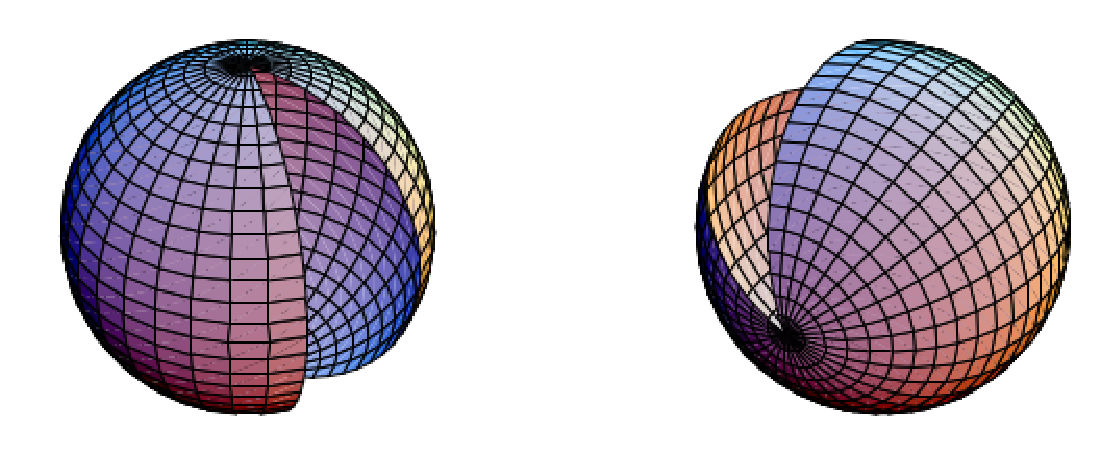
\includegraphics[scale=0.5]{Images_Fichiers/1.eps}
\end{figure}
  
\subsection[Métrique sur une surface]{\uline{Métrique sur une surface}}

\defibox{\ \\
Posons $E, F$ et $G$ les fonctions définies par : $E = ||x_u||^2$, $F = x_u.x_v$ et $G=||x_v||^2$, \\
où $x_u$ et $x_v$ représentent les dérivées selon $u$ et $v$ du patch $x$. \\
Alors la \uline{métrique Riemannienne} induite sur la surface est la forme différentielle donnée par :
$$ds^2 = E\ du^2 + 2F\ du\ dv + G\ dv^2$$
}
\begin{figure}[h!]
      \centering 
      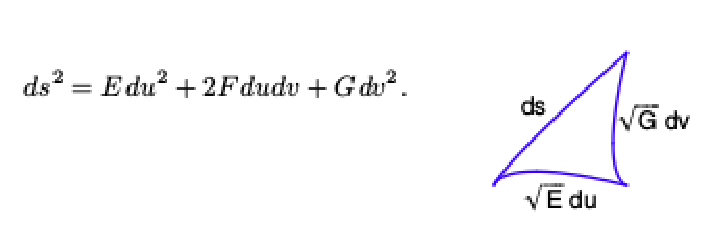
\includegraphics[scale=0.5]{Images_Fichiers/1b.eps}
\end{figure}

On peut voir ça comme une variante infinitésimale du théorème de Pythagore appliqué sur une surface : 

\begin{figure}[h!]
      \centering 
      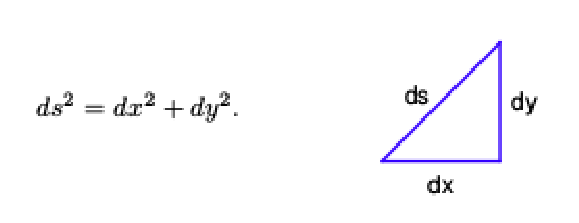
\includegraphics[scale=0.5]{Images_Fichiers/1a.eps}
\end{figure}

\subsection[Aire d'une surface]{\uline{Aire d'une surface}}


\defibox{Soit $\mathscr{R}$ une partie compacte d'une surface, et soit $x:\mathscr{U} \rightarrow \R^3$ un patch dont l'image est $\mathscr{R}$. Alors \uline{l'aire de $\mathscr{R}$} est égale à $$A = \iint_{x^{-1}(\mathscr{R})}\sqrt{EG-F^2}\ du\ dv.$$ De plus, ce nombre est indépendant du patch choisi. Si $\mathscr{R}$ est une union de plusieurs patchs disjoints, l'aire de $\mathscr{R}$ est la somme des aires de chaque patch. }

Intuitivement, $\mathscr{U}$ est composé de carrés infinisimaux dont les cotés sont ont pour mesure $du$ et $dv$. Son aire $dA$ est donnée par $du\ dv$.\\
Un carré infinitésimal est transformé par $x$ en un parallélograme infinitésimal de coté $x_u$ et $x_v$. 
On peut montrer que $$\sqrt{EG-F^2}=||x_u||\cdot ||x_v||\cdot sin\ \theta,$$ où $\theta$ est l'angle entre $x_u$ et $x_v$. \\
Donc $\sqrt{EG-F^2}$ est l'aire d'un parallélogramme infinitésimal.\\
Pour obtenir l'aire totale, on intègre toutes ces aires infinitésimales.

\section[Définition]{\uline{Définition}}

\subsection[Courbure normale]{\uline{Courbure normale}}

\defibox{Soit $u_p$ un vecteur unitaire tangent à une surface $\mathscr{M}$ en un point $p$.\\
On appelle \uline{courbure normale de $\mathscr{M}$ dans la direction $u_p$} le nombre réel
$$k(u_p)=(-D_{u_p}\cdot U)\cdot u_p, $$
où $U$ est un champ de vecteur normal à $\mathscr{M}$. \\
Le nombre $D_{u_p}\cdot U$ représente la dérivée du champ de vecteur $U$ dans la direction $u_p$. Il sera noté $D_{u}\cdot U$ si le point $p$ est clair. }

Plus concrètement, si $k(u_p)>0$ (resp. $k(u_p)<0$) alors, en suivant la direction $u_p$, $\mathscr{M}$ se courbe dans la même direction que le vecteur normal $U(p)$ (resp. dans la direction opposée).
Sur le schéma ci-dessous, nous voyons que la surface ci-dessous a une courbure négative selon le vecteur $u_1$, et une positive selon le vecteur $u_2$ : 

\begin{figure}[h!]
      \centering 
      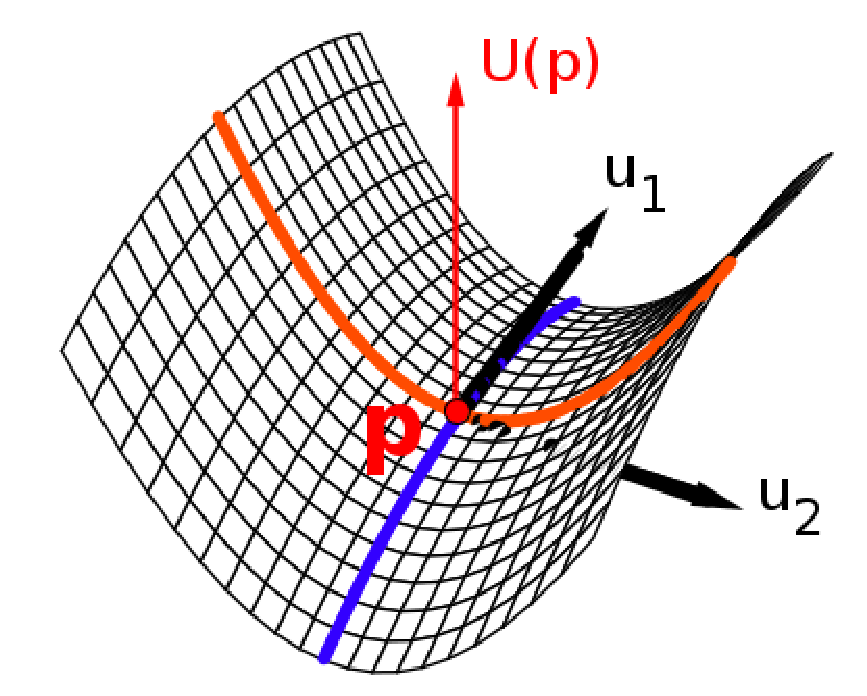
\includegraphics[scale=0.3]{Images_Fichiers/2a.eps}
\end{figure}

\subsection[Surface minimale]{\uline{Surface minimale}}

Pour un point $p$ donné, il existe deux nombres $k_1$ et $k_2$, appelés courbures principales de $\mathscr{M}$ en $p$ qui sont respectivement le maximum et le minimum des courbures normales de $\mathscr{M}$ au point $p$ pour $u_p$ parcourant l'ensembles des vecteurs unitaires tangents à $p$.

\begin{figure}[h!]
      \centering 
      \legend{}
      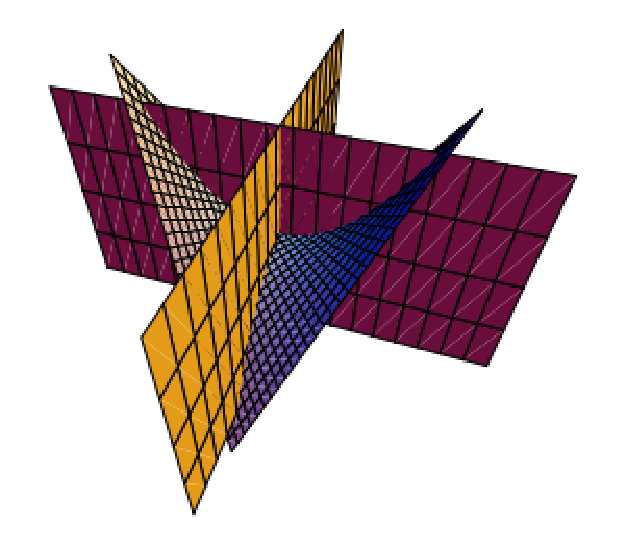
\includegraphics[scale=0.5]{Images_Fichiers/2.eps}
\end{figure}
Sur ce dessin, le point $p$ est à l'intersection de la surface et des plans violet et jaune. 
Supposons que le champ de vecteurs $U$ pointe vers le dessus de la surface. Le vecteur tangent dont la direction donne la courbure maximale est donc dans le plan violet et celui qui donne la courbure minimale est dans le plan jaune.

\defisbox{\ \\
$\bullet$ $\frac{k_1+k_2}{2}$ est la \uline{courbure moyenne} de la surface en $p$.\\
$\bullet$ Une \uline{surface minimale} est une surface pour laquelle en tout point le nombre $H$ vaut 0.}

D'après la définition d'une surface minimale, on a donc en chaque point d'une telle surface, la courbure maximale qui est égale à l'opposé de la courbure minimale. 

\subsection[Exemples de surfaces minimales]{\uline{Exemples de surfaces minimales}}

Dans cette partie, nous donnerons quelques exemples de surfaces minimales les plus courantes, ainsi qu'une paramétrisation. 

Pour démontrer que la surface est bien minimale, il faut utiliser des formules sur le calcul de la courbure moyenne qui utilisent les expressions explicites de $E$, $F$, et $G$, ainsi que des quantités $f$, $g$, $h$ qui sont issues des dérivées secondes de $x(u,v)$. Ces calculs étant purement techniques, nous ne les reproduisons pas ici.

\subsubsection[Le caténoïde]{\uline{Le caténoïde}}

Pour $a$ un réel positif, la surface paramétrée par $x(u,v) = (a\ cos\ u\ cosh\ v, a\ sin\ u\ cosh\ v, a\ v)$ est une surface minimale, appelée caténoïde. Historiquement c'est la première surface minimale non plane, elle a été découverte par Leonhard Euler en 1744. Dans la suite, je parlerai de caténoïde dans le cas $a=1$, sauf mention contraire.

\begin{figure}[h!]
      \centering 
      \legend{Un caténoïde}
      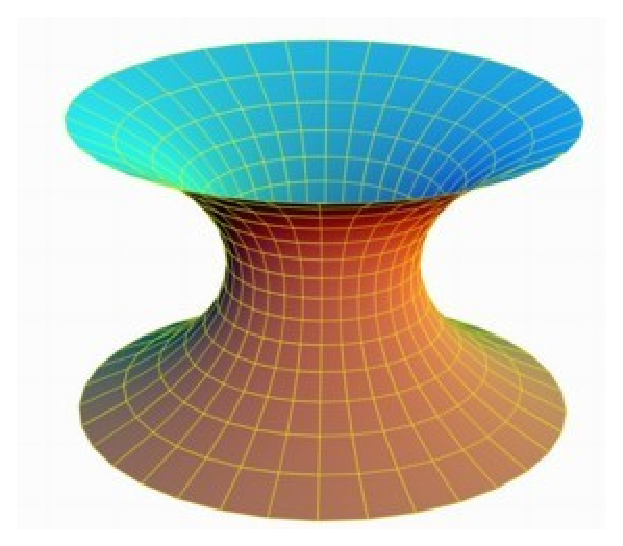
\includegraphics[scale=0.5]{Images_Fichiers/3.eps}
\end{figure}

\subsubsection[L'hélicoïde]{\uline{L'hélicoïde}}

La surface paramétrée par $x(u,v) = (v\ cos\ u, v\ sin\ u, u)$ est une surface minimale, appelée hélicoïde . Elle a été découverte par Jean-Baptiste Marie Charles Meusnier de la Place en 1776.

\begin{figure}[h!]
      \centering 
      \legend{Un hélicoïde}
      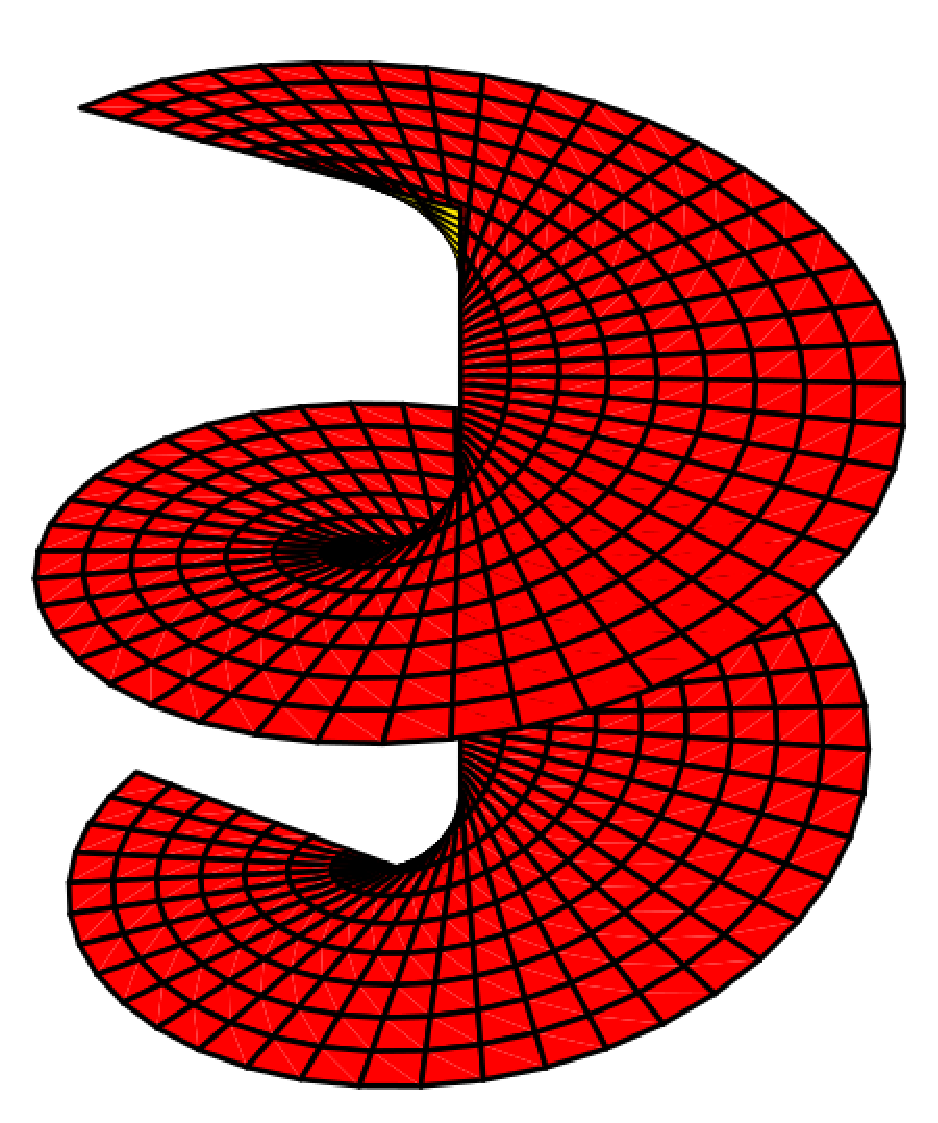
\includegraphics[scale=0.25]{Images_Fichiers/4.eps}
\end{figure}

\subsubsection[La surface d'Enneper]{\uline{La surface d'Enneper}}

La surface paramétrée par $x(u,v) = \left(u - \frac{u^3}{3} + u v^2, v-{\frac {v^{3}}{3}}+vu^{2}, u^2-v^2\right)$ est une surface minimale. Elle a été découverte par Alfred Enneper en 1863. \\On voit que cette surface présente des auto-intersections.

\begin{figure}[h!]
      \centering 
      \legend{La surface d'Enneper}
      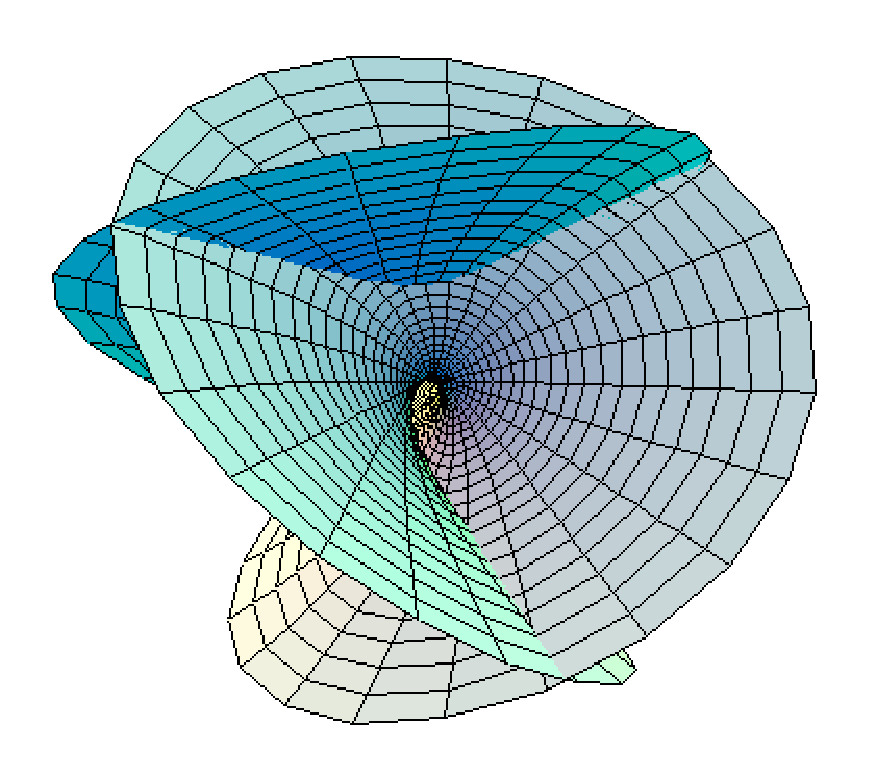
\includegraphics[scale=0.5]{Images_Fichiers/5.eps}
\end{figure}


\subsubsection[Transformation d'hélicoïde en caténoïde]{\uline{Transformation d'hélicoïde en caténoïde}}

La transformation $z$ définie pour $0\leq t \leq \frac{\pi}{2}$ et pour tout $(u,v)\in\mathscr{U}$ par $$z_{u,v}(t) = cos\ t(sinh\ v\ sin\ u, -sinh\ v\ cos\ u, u)+sin\ t(cosh\ v\ cos\ u, cosh\ v\ sin\ u, v)$$ donne pour chaque $t$ une surface minimale et pour $t=0$, un hélicoïde, et pour $t=\frac{\pi}{2}$ un caténoïde. 

Nous verrons plus tard, dans le chapitre Weierstrass, que ce genre de déformation existe pour toutes les surfaces minimales.

Voici un exemple de ces déformations :\\
\begin{center}
\animategraphics[autoplay,loop,width=8cm]{2}{Images_Fichiers/HelicoideDeformee/helicoideDeformee-}{0}{6} 
\end{center}

\section[Une autre approche]{\uline{Une autre approche}}

Nous allons maintenant voir une autre façon de définir les surfaces minimales, et du même coup expliquer leur nom. Intuitivement, une surface minimale (bornée) est la surface ayant une aire minimale parmi toutes celles "légèrement déformées" ayant le même bord. Donc si on déforme légèrement l'intérieur d'une surface minimale, la surface obtenue a une aire plus grande. \\
Précisons cela : 

Soit $x:\mathscr{U}\rightarrow \mathscr{M}$ un patch régulier et soit $\mathscr{Q}$ une partie bornée de $\mathscr{U}$ : 

\defin{Soient $U$ un champ de vecteurs unitaires normaux à $\mathscr{M}$  , $h:\mathscr{Q}\rightarrow \R$ une application différentiable, et $\epsilon > 0$. \\
Alors la \uline{variation normale de $x$} définie par $h$ est l'application 
$X:]-\epsilon , \epsilon[\times \mathscr{Q} \rightarrow \R^3$ t.q. : 
$$ X(t, (u,v)) = x(u,v)+t\cdot h(u,v)U(u,v)$$
On note $X_t:\mathscr{Q} \rightarrow \R^3$ l'application définie pour $-\epsilon < t < \epsilon$ par $X_t(u,v) = X(t,(u,v))$ et $A:]-\epsilon, \epsilon[\rightarrow \R^+$ celle définie par $A(t)=A(X_t)$, qui représente l'aire de la surface $X_t$.}

L'application $t\mapsto X_t$ représente donc une déformation continue de la surface $X_0=x$, chaque point étant éloigné perpendiculairement de cette surface.

\theobox{$x$ est minimale sur $\mathscr{Q}$ si et seulement si pour toute fonction différentiable $$h:\mathscr{Q} \rightarrow \R,\ A'(0)=0.$$}

\uline{Remarque} : On retombe sur la notion intuitive : \\
Si la différentielle de l'aire s'annule, cela signifie que l'aire aura atteint un minimum local. Donc une surface minimale est une surface d'aire minimale parmi toutes les surfaces "proches". 

Attention, une surface minimale n'est pas forcément d'aire minimale : \\
Par exemple, (information trouvée sur le site mathcurve), pour les bords étant deux cercles de même dimension (sur le dessin ci-dessous, sur une vue en coupe, ces cercles sont représentés en noir), on peut construire trois surfaces minimales : un caténoïde (en rouge), un "pseudo-caténoïde" (en gris), et la surface de Goldbach, constituée seulement des deux disques dans les cercles (donc en noir aussi sur le dessin).

\begin{figure}[h!]
      \centering 
      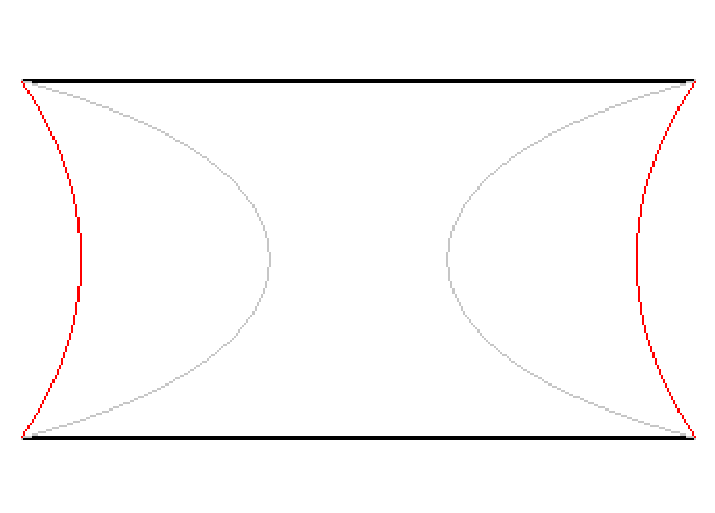
\includegraphics[scale=0.5]{Images_Fichiers/3a.eps}
      \legend{Trois surfaces minimales}
\end{figure}

Ici, seule le caténoïde rouge est d'aire minimale, les autres surfaces sont des minimums locaux.

\uline{Idée de la démonstration} : 

On a $A(t) = \iint_{\mathscr{Q}}\sqrt{E(t)G(t)-F^2(t)}\ du \ dv$, où $E(t)$ (resp. $F(t)$, $G(t)$) est le nombre $E$ (resp. $F$, $G$) de la surface $X_t$.\\
Après calcul, grâce à la définition, on montre que $E(t)=E + 2th x_u \cdot U_u + O(t^2)$, et des égalités similaires pour $F(t)$ et $G(t)$, puis que 
$$A(t)= \iint_\mathscr{Q}\sqrt{EG-F^2}du\ dv - 2t\iint\mathscr{Q}hH\sqrt{EG-F^2}\ du\ dv + O(t^2),$$ où $H$ est la courbure moyenne de la surface.
Il ne reste plus qu'à calculer : $$A'(0) = - 2\iint_\mathscr{Q}h\cdot H\sqrt{EG-F^2}\ du\ dv $$
Il est alors évident que si $H = 0$, alors $A'(0)=0$. 

Réciproquement, raisonnons par l'absurde : \\
Supposons que $A'(0)=0$ pour toute fonction $h$, et qu'il existe $q$ tel que $H(q)\neq 0$. On choisit alors un petit voisinage $\mathscr{V}$ de $q$ sur lequel $H$ est de signe constant, et on choisit alors une fonction $h$ comme étant nulle en-dehors de $\mathscr{V}$, valant $H(q)$ en $q$, et du même signe que $H(q)$ sur $\mathscr{V}$. \\
Avec ces conditions, on a alors $hH>0$ sur $\mathscr{V}$, et donc $A'(0)<0$, ce qui contredit l'hypothèse de départ. 

L'équivalence est donc bien prouvée.

\chapter[Le problème de Plateau]{\uline{Le problème de Plateau}}

Le problème de Plateau est le problème qui consiste à trouver, à partir d'une ou plusieurs courbes fermées représentant les bords d'une surface, la (ou les) surfaces minimales possédant ces courbes comme bord. Ce problème fut posé par Lagrange dès 1760, et porte le nom de Joseph Plateau qui s'intéressa à ce problème en étudiant des bulles de savon. 

Le problème a été résolu en 1931 par Jesse Douglas, qui obtenut alors la médaille Fields. Selon le type et le nombre de courbes considérées, il peut y avoir une ou plusieurs surfaces minimales ayant ces courbes comme bord, mais toujours en nombre fini. Une seule de ces surfaces a une aire minimale, et celle-ci n'a pas d'auto-intersection. Le problème est que même s'il est prouvé que la surface d'aire minimale existe, il peut être compliqué de la construire.

Dans la suite, j'ai donc implémenté l'algorithme proposé par Ulrich Pinkall et Konrad Polthier dans un article de février 1993, "Computing Discrete Minimal Surfaces and Their Conjuguates". 

\section[Description de l'algorithme]{\uline{Description de l'algorithme}}

\defibox{\ \\
$\bullet$ Une surface discrète est une surface constituée de triangles, (éventuellement dégénérés en un segment ou un point).\\
$\bullet$ Une surface discrète est minimale ssi n'importe quelle petite perturbation d'un des sommets non situé sur un bord augmente l'aire de la surface}

L'algorithme est un algorithme itératif. Il prend en entrée un ensemble $\Gamma$ non vide constitué de courbes correspondant aux bords (ces courbes étant en fait constituées de segments de droites), et une surface discrète quelconque ayant $\Gamma$ comme frontière. 
Il renvoie en sortie une approximation d'une surface minimale de frontière $\Gamma$.

Pour ce faire, on va parcourir tous les points intérieurs à la surface de départ (ceux de la surface qui ne sont pas dans $\Gamma$), et on remplace ce point par le point $p$ obtenu par la formule suivante $$p=\frac{\sum (cot\ \alpha_i + cot\ \beta_i)q_i}{\sum cot\ \alpha_i + cot\ \beta_i}, $$ les sommes portant sur tous les points $q_i$ voisins du point considéré. 
Les angles $\alpha_i$ et $\beta_i$ sont les angles opposés au segment $a_i$ reliant le point $p$ au sommet $q_i$, comme schématisé ci-dessous : 

\begin{figure}[h!]
      \centering 
      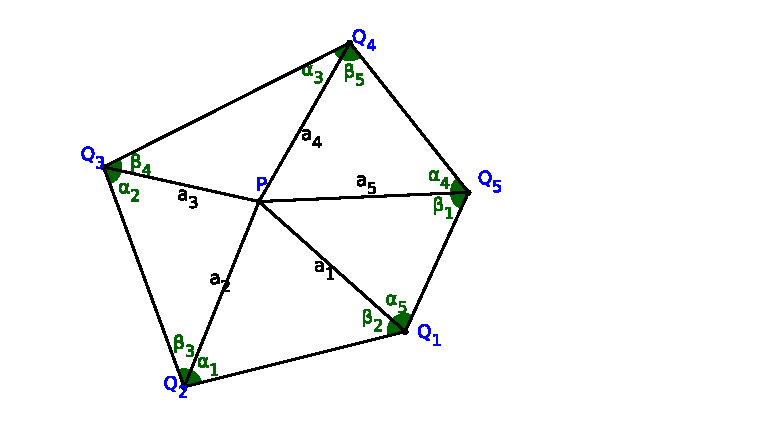
\includegraphics[scale=1]{Images_Fichiers/6.eps}
\end{figure}

On obtient donc une nouvelle surface plus proche de la surface minimale cherchée que celle de départ. On répète ce processus ensuite plusieurs fois soit avec un nombre d'itérations donné, soit jusqu'à que la différence entre l'aire de deux surfaces successives soit plus petite qu'un paramètre $\epsilon >0$ donné. 

A la $i-ème$ itération, nous construisons donc une fonction $f_i$ qui transforme chaque triangle $\Delta_{1,i}$ de la surface en cours de traitement en un triangle $\Delta_{2,i}$ de la nouvelle surface.

A la fin, nous obtenons une surface très proche de la surface minimale cherchée si le nombre d'itérations est suffisant.

\section[Explication de l'algorithme]{\uline{Explication de l'algorithme}}

L'idée est non pas d'essayer de minimiser l'aire de la surface de départ $x:\mathscr{U}\rightarrow \R^3$ , mais celle de l'énergie de $f$, $E_D(f)$, donnée par $$E_D(f) = \frac{1}{2} \int_\mathscr{U} |\nabla f|^2 \text{ avec } |\nabla f|^2 = tr(^t\partial f \cdot \partial f),$$
où $f$ est une fonction qui perturbe légèrement notre surface de départ.\\
D'après l'article, ceci est équivalent, et fait aboutir les calculs. 

Le tout repose sur une propriété importante, dont je ne donnerai pas la démonstration complète ici :

\proprbox{Soit $f$ une application linéaire entre deux triangles $\Delta_1$ et $\Delta_2$. Alors son énergie est donnée par : $$E_D(f) = \frac{1}{4}\sum_{i=1}^{3}cot\ \alpha_i\cdot |a_i|^2,$$ où les $\alpha_i$ sont les angles du triangle $\Delta_1$, et $a_i$ l'image dans $\Delta_2$ du côté opposé à $\alpha_i$. }

La démonstration, assez technique, repose sur la séparation de $f$ en $f=\psi \circ \varphi^{-1}$ avec $\varphi : \Delta \rightarrow \Delta_1$ et $\psi : \Delta \rightarrow \Delta_2$ les applications qui envoient la base canonique $(e_1,e_2)$ sur deux côtés de $\Delta_1$ pour $\varphi$, de $\Delta_2$ pour $\psi$, $\Delta$ étant le triangle formé par $e_1$ et $e_2$.\\
On a alors $\partial f = \partial \psi \partial \varphi^{-1}$\\
On démontre ensuite par le calcul que $tr(^t\partial f \cdot \partial f) = \frac{1}{det\ \partial \varphi}\sum_{i=1}^{3} cot\ \alpha_i|a_i|^2$, et on en déduit que $E_D(f) = \frac{1}{2} \int_\Delta tr(^t\partial f \cdot \partial f) det\ \partial \varphi^{-1}$, soit comme l'aire de $\Delta$ est $\frac{1}{2}$, $$E_D(f) = \frac{1}{4}\sum_{i=1}^{3} cot\ \alpha_i\cdot |a_i|^2.$$

\defibox{Pour une application $f$ entre deux surfaces discrètes, l'énergie de $f$ est la somme des énergies de chaque restriction de $f$, notées $f_i:\Delta_{1,i} \rightarrow \Delta_{2,i}$ où les $\Delta_{2,i}$ sont les triangles images de $\Delta_{1,i}$ par $f$.} 

Donc, pour une fonction $f$ entre deux surfaces discrètes $T_1$ et $T_2$, on a 
$$E_D(f) = \sum_{i=1}^{\#triangles} E_D(f_i) = \frac{1}{4}\sum_{i=1}^{\#bords} (cot\ \alpha_i + cot\ \beta_i) |a_i|^2.$$
Dans la dernière expression, la somme a été faite sur les bords plutôt que sur les triangles, ce qui permet de regrouper pour chaque arête, les deux angles adjacents $\alpha_i$ et $\beta_i$.

Il ne reste plus qu'à chercher quand la dérivée s'annule pour une surface minimale, c'est-à-dire résoudre $\frac{\partial}{\partial p}E_D(f) = 0$. \\
D'après la formule précédente sur $E_D(f)$, cette équation devient 
$$\frac{1}{2}\sum_{i=1}^{\#\text{voisins de }p} (cot\ \alpha_i + cot\ \beta_i) (p-q_i) = 0$$
Ce qui donne, en isolant $p$ : 
$$\boxed{p=\frac{\sum_{i=1}^{\#\text{voisins de }p}(cot\ \alpha_i + cot\ \beta_i) q_i}{\sum_{i=1}^{\#\text{voisins de }p}cot\ \alpha_i + cot\ \beta_i}}$$

Si tous les points $p$ de la surface vérifient cette formule, alors la surface est minimale. L'algorithme consiste donc à remplacer tous les points $p$ par le point vérifiant la formule ci-dessus, et à continuer.

\section[Implémentation]{\uline{Implémentation}}

J'ai crée une classe Plateau, chaque objet de cette classe aura deux attributs, le nombre d'itération à faire, et un ensemble de points du maillage de départ (les bords).\\
Je crée ensuite une liste de triplets représentant tous les triangles de la surface de base, surtout nécessaire si le maillage de départ est carré et non triangulaire.

Ensuite, je crée un dictionnaire qui à partir d'une arête, renvoie une liste constituée de quatre points : les deux points de cette arête et chaque point formant un triangle avec cette arête (s'il n'y en a qu'un, le quatrième objet de la liste est "null").

Puis, à chaque itération, je crée un nouveau dictionnaire, qui à partir de chaque arête $a_i$, renvoie le coefficient $cot\ \alpha_i + cot\ \beta_i$ comme ceci : 
\begin{lstlisting}[frame=single, framerule=0pt]
for (let j = 0; j < this.nbIterations; j++) {
	let LineToCoeff = new StringMap<number>()
	for (let key of dicoEdgeTo4Vertex.allKeys()) {
		let s1 = dicoEdgeTo4Vertex.getValue(key)[0]
		let s2 = dicoEdgeTo4Vertex.getValue(key)[1]
		let s3 = dicoEdgeTo4Vertex.getValue(key)[2]
		let s3Bis = dicoEdgeTo4Vertex.getValue(key)[3]
		if (s3Bis != null) {
			LineToCoeff.putValue(key,
				1 / Math.tan(geo.angleBetweenTwoVectorsBetween0andPi(
					XYZ.newFrom(s1.position).substract(s3.position),
					XYZ.newFrom(s2.position).substract(s3.position))) +
				1 / Math.tan(geo.angleBetweenTwoVectorsBetween0andPi(
					XYZ.newFrom(s1.position).substract(s3Bis.position),
					XYZ.newFrom(s2.position).substract(s3Bis.position))))
		}
	}
\end{lstlisting}

et je stocke dans une liste chaque nouvelles coordonnées des différents points : 

\begin{lstlisting}[frame=single, framerule=0pt]
	let newPositionsVertices = []
    for (let vertex of insidePoints) {
		let newPosition = new XYZ(0, 0, 0)
		let sumCoeffs = 0
		for (let link of vertex.links) {
			let id1 = Math.min(vertex.hashNumber, link.to.hashNumber)
			let id2 = Math.max(vertex.hashNumber, link.to.hashNumber)
			let coeff = LineToCoeff.getValue(id1 + "," + id2)
			newPosition.add(XYZ.newFrom(link.to.position).scale(coeff))
			sumCoeffs += coeff
		}
		newPosition.scale(1. / sumCoeffs)
		newPositionsVertices.push(newPosition)
	}
\end{lstlisting}

A la fin, je change point par point les coordonnées de chaque point en les remplaçant par les nouvelles : 

\begin{lstlisting}[frame=single, framerule=0pt]
	let i = 0
	for (let vertex of insidePoints) {
		vertex.setPosition(newPositionsVertices[i].x, newPositionsVertices[i].y,
			newPositionsVertices[i].z)
		i += 1
	}
}
\end{lstlisting}

\section[Résultats]{\uline{Résultats}}

\subsection[Caténoïde]{\uline{Caténoïde}}

Je pars d'un cylindre, et je fixe les deux cercles qui forment son bord. En appliquant l'algorithme, on constate bien que le cylindre se déforme progressivement en caténoïde. 
Voici une animation qui montre celà pour différentes valeurs entre $0$ et $1000$ itérations : 

\begin{center}
\animategraphics[autoplay,loop,width=12cm]{2}{Images_Fichiers/catenoide/catenoide-}{0}{9} 
\end{center}

En repensant aux bulles de savon (une surface minimale est théoriquement la forme prise par un film de savon dont les bords en fil de fer ont été trempés), on imagine bien que si on fabrique deux cercles en fil de fer qu'on trempe dans une eau savonneuse, en les écartant, un caténoïde se formera au début, puis quand on écartera trop, le caténoïde cassera pour ne laisser que deux disques de savon entre les fils de fer. 

Quand ce caténoïde cassera-t-il ?

\noindent Tout simplement quand l'aire des deux cercles sera inférieure à l'aire du caténoïde formé entre les deux cercles. 

Nous allons donc relancer notre algorithme avec un rayon des cercles deux fois plus petit et regarder ce que donne l'algorithme :
\newpage

\begin{figure}[h!]
   \begin{minipage}[b]{0.30\linewidth}
 	  \legend{300 itérations}      
      \centering 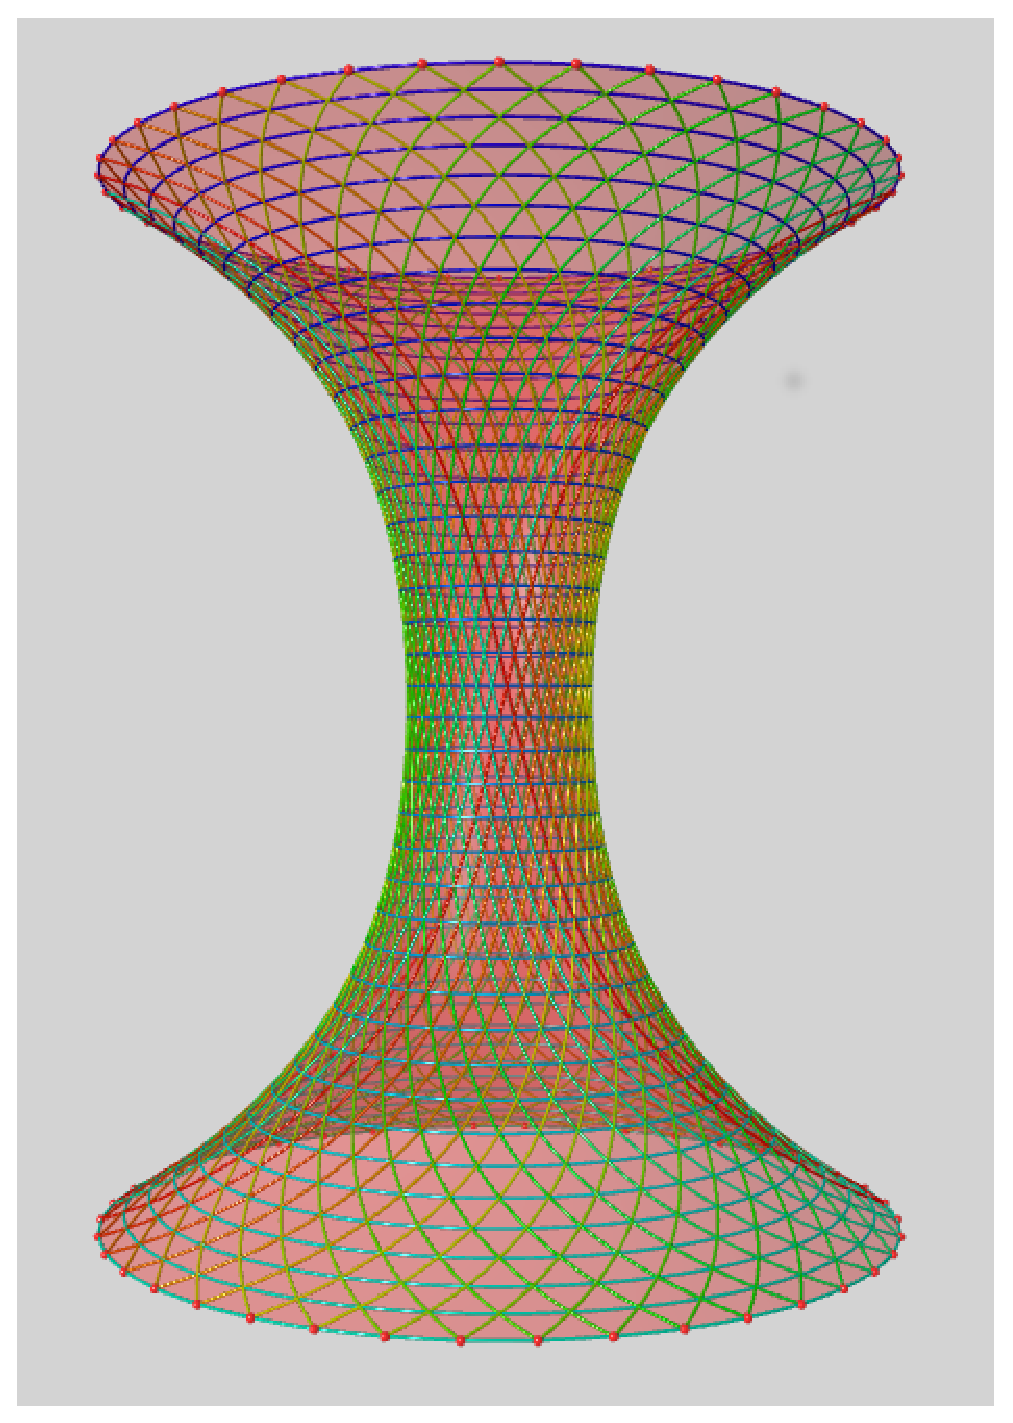
\includegraphics[scale=0.2]{Images_Fichiers/7.eps}
     
   \end{minipage}\hfill
   \begin{minipage}[b]{0.3\linewidth}   
	 \legend{500 itérations}     
     \centering 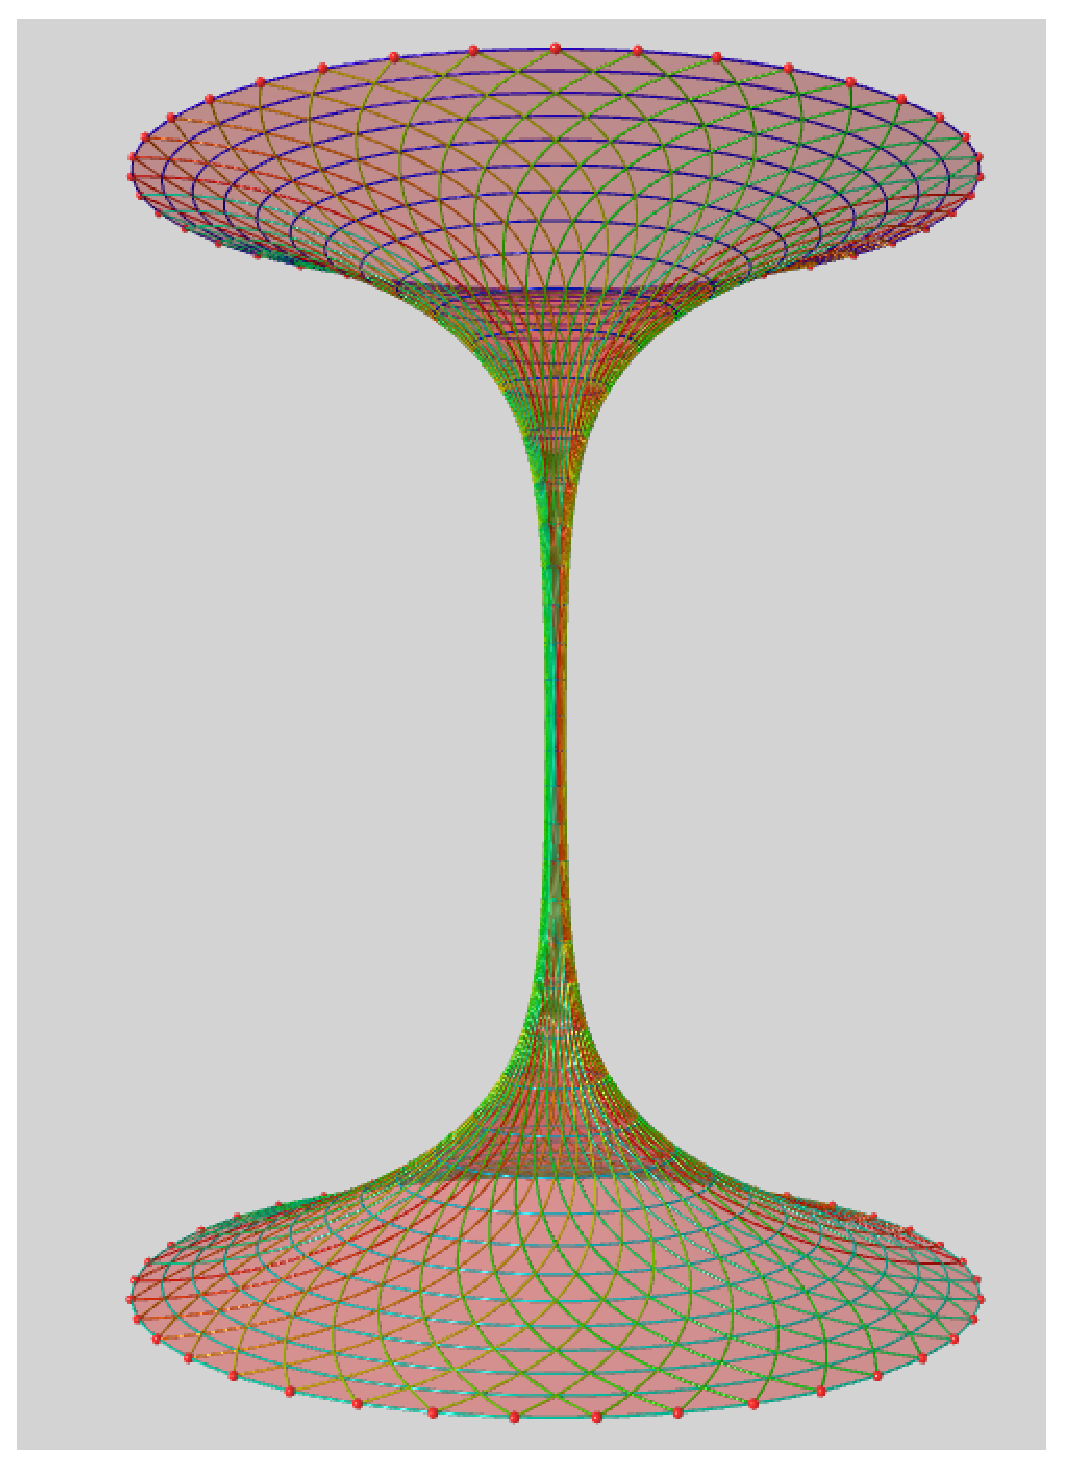
\includegraphics[scale=0.197]{Images_Fichiers/8.eps}
      
   \end{minipage}\hfill
   \begin{minipage}[b]{0.3\linewidth}   
     \legend{1000 itérations}     
     \centering 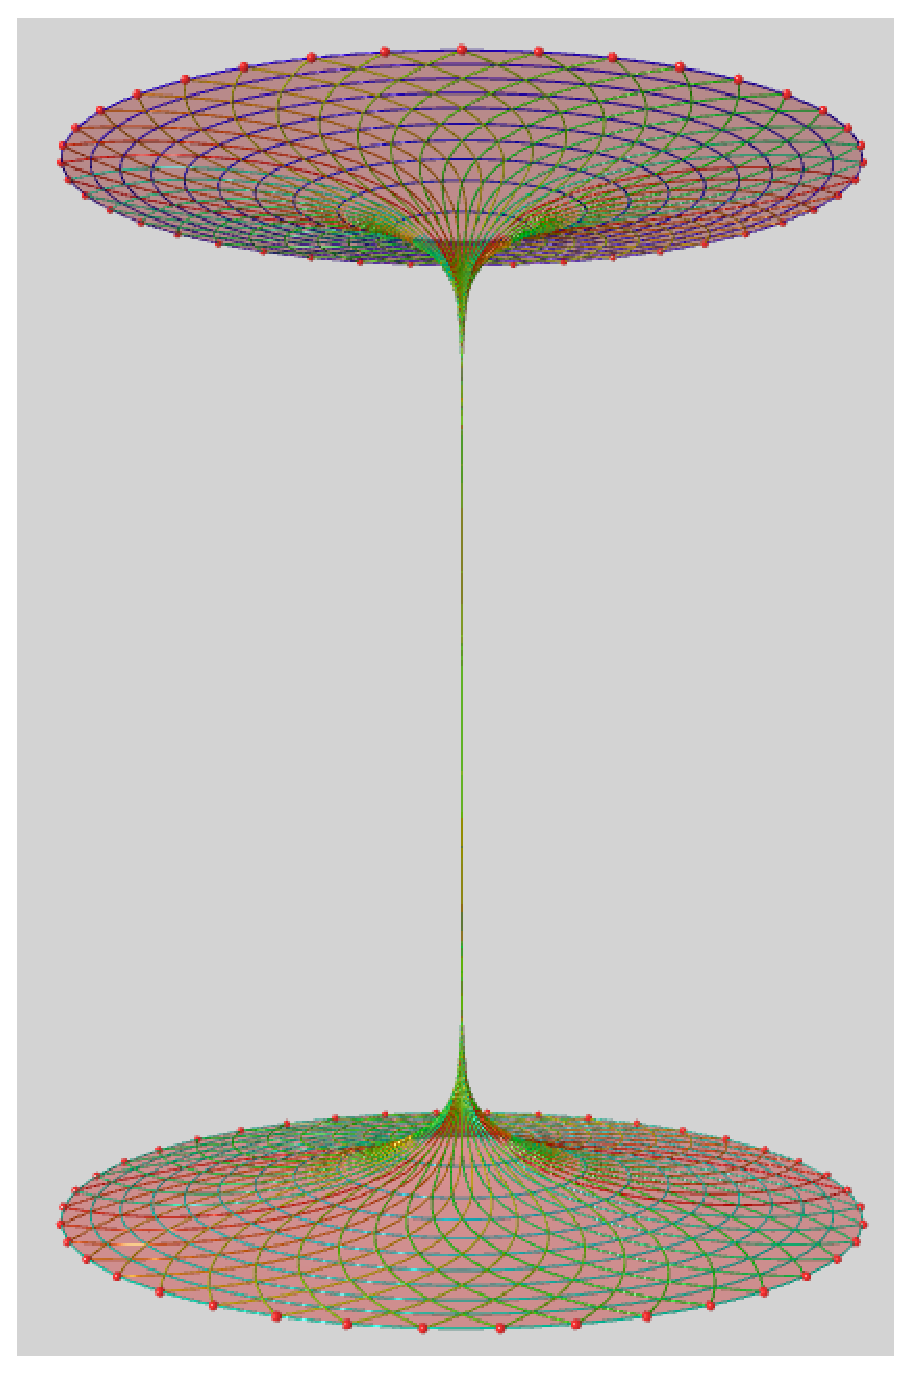
\includegraphics[scale=0.206]{Images_Fichiers/9.eps}
     
   \end{minipage}
\end{figure}

Les résultats sont donc bien conformes à ce qu'on pourrait attendre. On pourrait également améliorer l'algorithme en supprimant les triangles trop dégénérés, ainsi, il ne resterait que les deux disques attendus.

\subsection[Surface de Riemann]{\uline{Surface de Riemann}}

La surface de Riemann est la surface minimale dont les bords sont constitués d'un carré, et de deux cercles, placés alternativement au-dessus et en dessous du carré. Ces bords sont représentés par les sommets en rouge sur le dessin ci-dessous.

J'ai donc créé deux cylindres (légèrement déformés pour ne pas avoir de problème de vecteur normal mal défini) dont chacun a une base dans le carré et l'autre dans un cercle. Voici le schéma de la surface de départ et celle après $20$ itérations de l'algorithme.\\

\begin{figure}[ht!]
      \centering 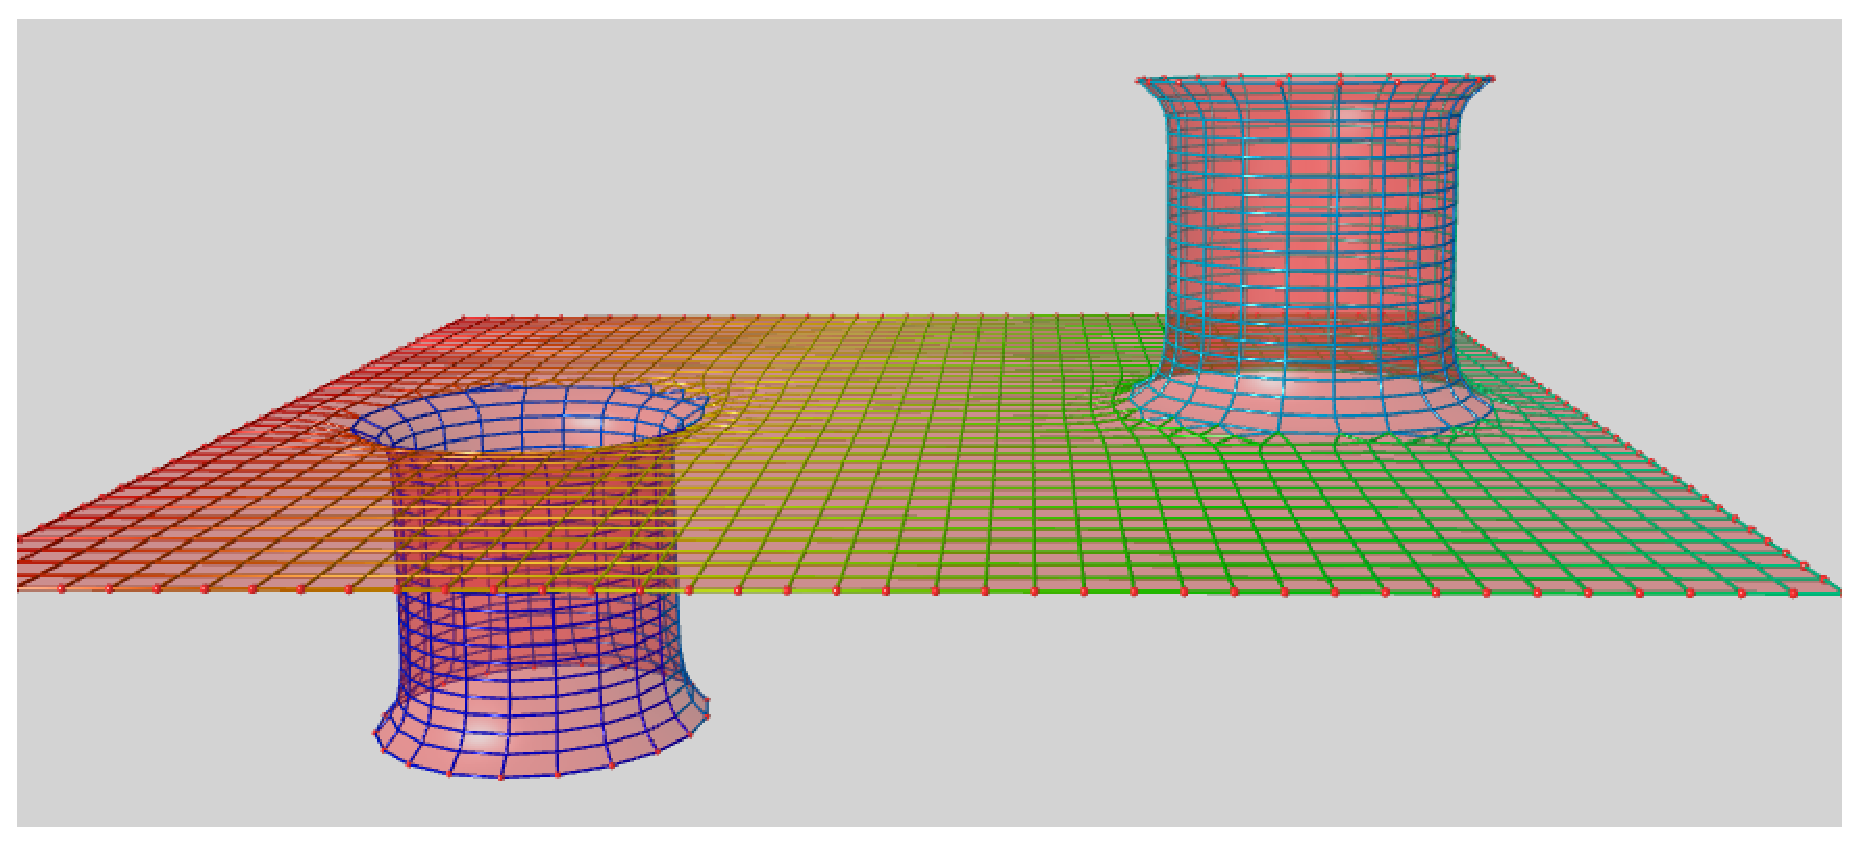
\includegraphics[scale=0.25]{Images_Fichiers/10.eps}
      \legend{Surface de départ}
\end{figure}
\  \vspace{-1cm} \\
\begin{figure}[ht!]
      \centering 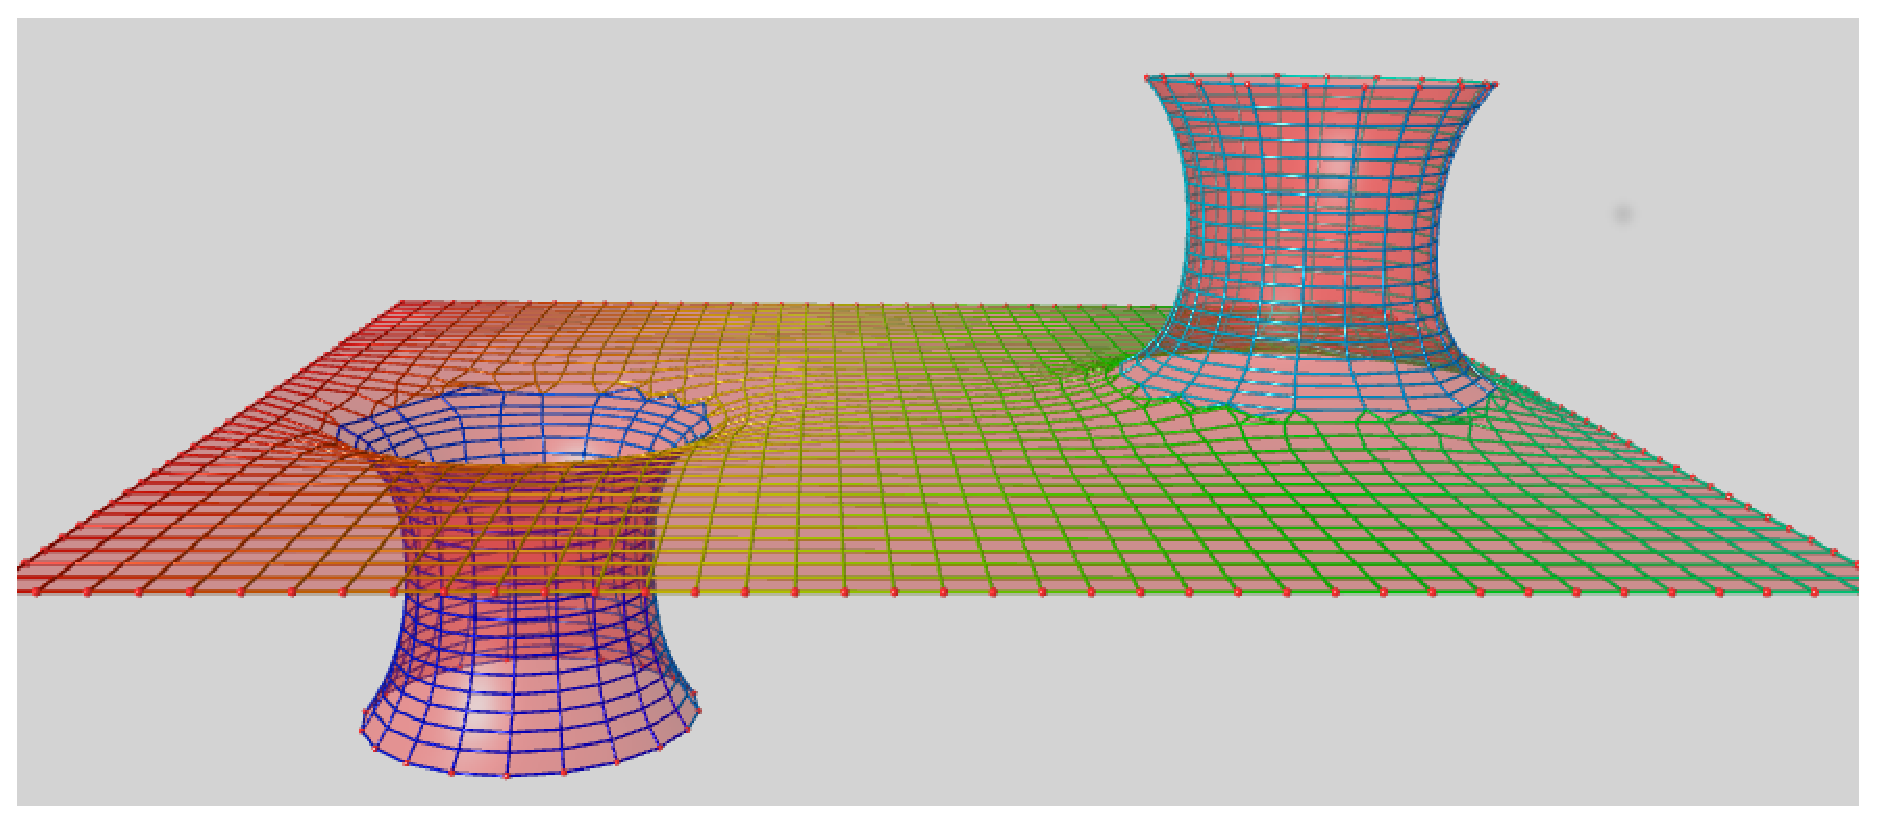
\includegraphics[scale=0.25]{Images_Fichiers/11.eps}
      \legend{20 itérations}
\end{figure}

\chapter[Représentation de Weierstrass-Enneper]{\uline{Représentation de Weierstrass-Enneper}}

La représentation de Weierstrass–Enneper est une formule liant le domaine des surfaces minimales à l'analyse complexe, découverte par Alfred Enneper et Karl Weierstrass dans les années 1860. 
Elle permet de trouver, à partir de deux fonctions complexes quelconques (ou presque), de trouver une surface minimale. On peut dès lors trouver une infinité de surfaces minimales.\\
Il est également remarquable que pour n'importe quelle surface minimale, il existe deux fonctions complexes dont la représentation de Weierstrass-Enneper avec ces fonctions donne la surface minimale. Plus précisément :

\theobox{Soit $x$ le patch d'une surface minimale. Alors il existe un domaine $D$ de $\C$, et deux fonctions $G : D\rightarrow \C$ et $h : D\rightarrow \C$ telles que :
\begin{enumerate}
\item $G$ et $h$ sont méromorphes sur $D$
\item $Gh$ est holomorphe sur $D$.
\end{enumerate}

Alors, pour $w\in \C$, la surface paramétrée par $$\Phi(w) = \Re \oint^w \left(
\frac{1}{2}\left(\frac{1}{G}-G\right)h, \frac{i}{2}\left(\frac{1}{G}+G\right)h, h\right) dz, $$où $\Re$ désigne la partie réelle, est minimale. \\
Inversement, toute surface minimale s'écrit sous cette forme. }
\newpage
\section[Implémentation]{\uline{Implémentation}}

J'ai commencé par modifier les formules ci-dessus pour ne plus avoir de division par un nombre complexe : 
$$\Phi(z) = \left(\Re \oint \varphi_1(z), \Re \oint \varphi_2(z), \Re \oint \varphi_3(z)\right), \text{ avec}$$

$$\begin{array}{cc}
\varphi_1(z) = & \frac{1}{2|G|^2}(\overline{G}-\overline{G}G^2)h\\
\varphi_2(z) = & \frac{i}{2|G|^2}(\overline{G}+\overline{G}G^2)h\\
\varphi_3(z) = & h\\
\end{array}
$$

N'ayant pas implémenté de classe complexe sur Typescript, j'ai codé un complexe comme une liste de deux réels (parties imaginaire et réelle), et ai codé des fonctions pour faire le produit complexe, l'addition et la soustraction.

La classe Weierstrass n'a qu'un attribut, le booléen $algebraicForm$ qui décide si les fonctions $G$ et $h$ sont rentrées sous les formes algébriques ou polaires, et le constructeur prend donc en entrée un maillage (l'ensemble des points $z$ de $\C$ qui auront une image par $\Phi$), et quatre fonctions qui représentent les parties entière et imaginaire de $G$ et $h$ (ou les modules et arguments selon la valeur de $algebraicForm$.

Avec tout ceci, je crée la fonction $CoordAIntegrer$, qui renvoie le triplet $\left(\varphi_1(z),  \varphi_2(z), \varphi_3(z)\right)$ d'après les notations ci-dessus, et je crée un dictionnaire qui à chaque sommet renvoie ce triplet appliqué au sommet.

Le but est de partir d'un sommet initial $P_0$, et de diviser la surface en différentes strates, chaque strate étant composée des sommets de distance donnée par rapport à $P_0$ (la distance entre deux points étant la longueur du plus petit chemin entre ces deux points).\\
A partir de cela, je crée un dictionnaire, qui à partir d'un sommet de distance $n$ de $P_0$, donne un des voisins de ce sommet qui est à distance $n-1$ (le sommet $P_0$ a pour valeur "null").

Enfin, je remplis un dictionnaire qui pour chaque sommet $w$ renvoie la valeur de l'intégrale curviligne sur le chemin entre $P_0$ et $w$. Pour ce faire, j'ajoute la valeur de l'intégrale trouvée pour le sommet voisin à la valeur trouvée par la méthode des milieux (c'est-à-dire pour deux voisins $w$ et $w'$, $\oint_w^{w'}f(z)dz \approx \frac{f(w)+f(w')}{2}\times (w'-w)$).
Il ne reste plus qu'à envoyer les points de $\C$ dans $\R^3$ par $\Phi$, et nous obtenons une surface minimale. 

\section[Résultats]{\uline{Résultats}}

J'ai créé un maillage plan circulaire autour de l'origine, où l'origine n'est pas dans le maillage, car pour des fonctions du type $z\mapsto \frac{1}{z}$, cela donne un pôle, et j'ai envoyé ces points dans $\R^3$ par l'algorithme précédent. 

\subsection[Un caténoïde]{\uline{Un caténoïde}}

Pour $G(z)=z$, et $h(z)=\frac{1}{z}$, on obtient le caténoïde : 

\begin{figure}[h!]
      \centering 
      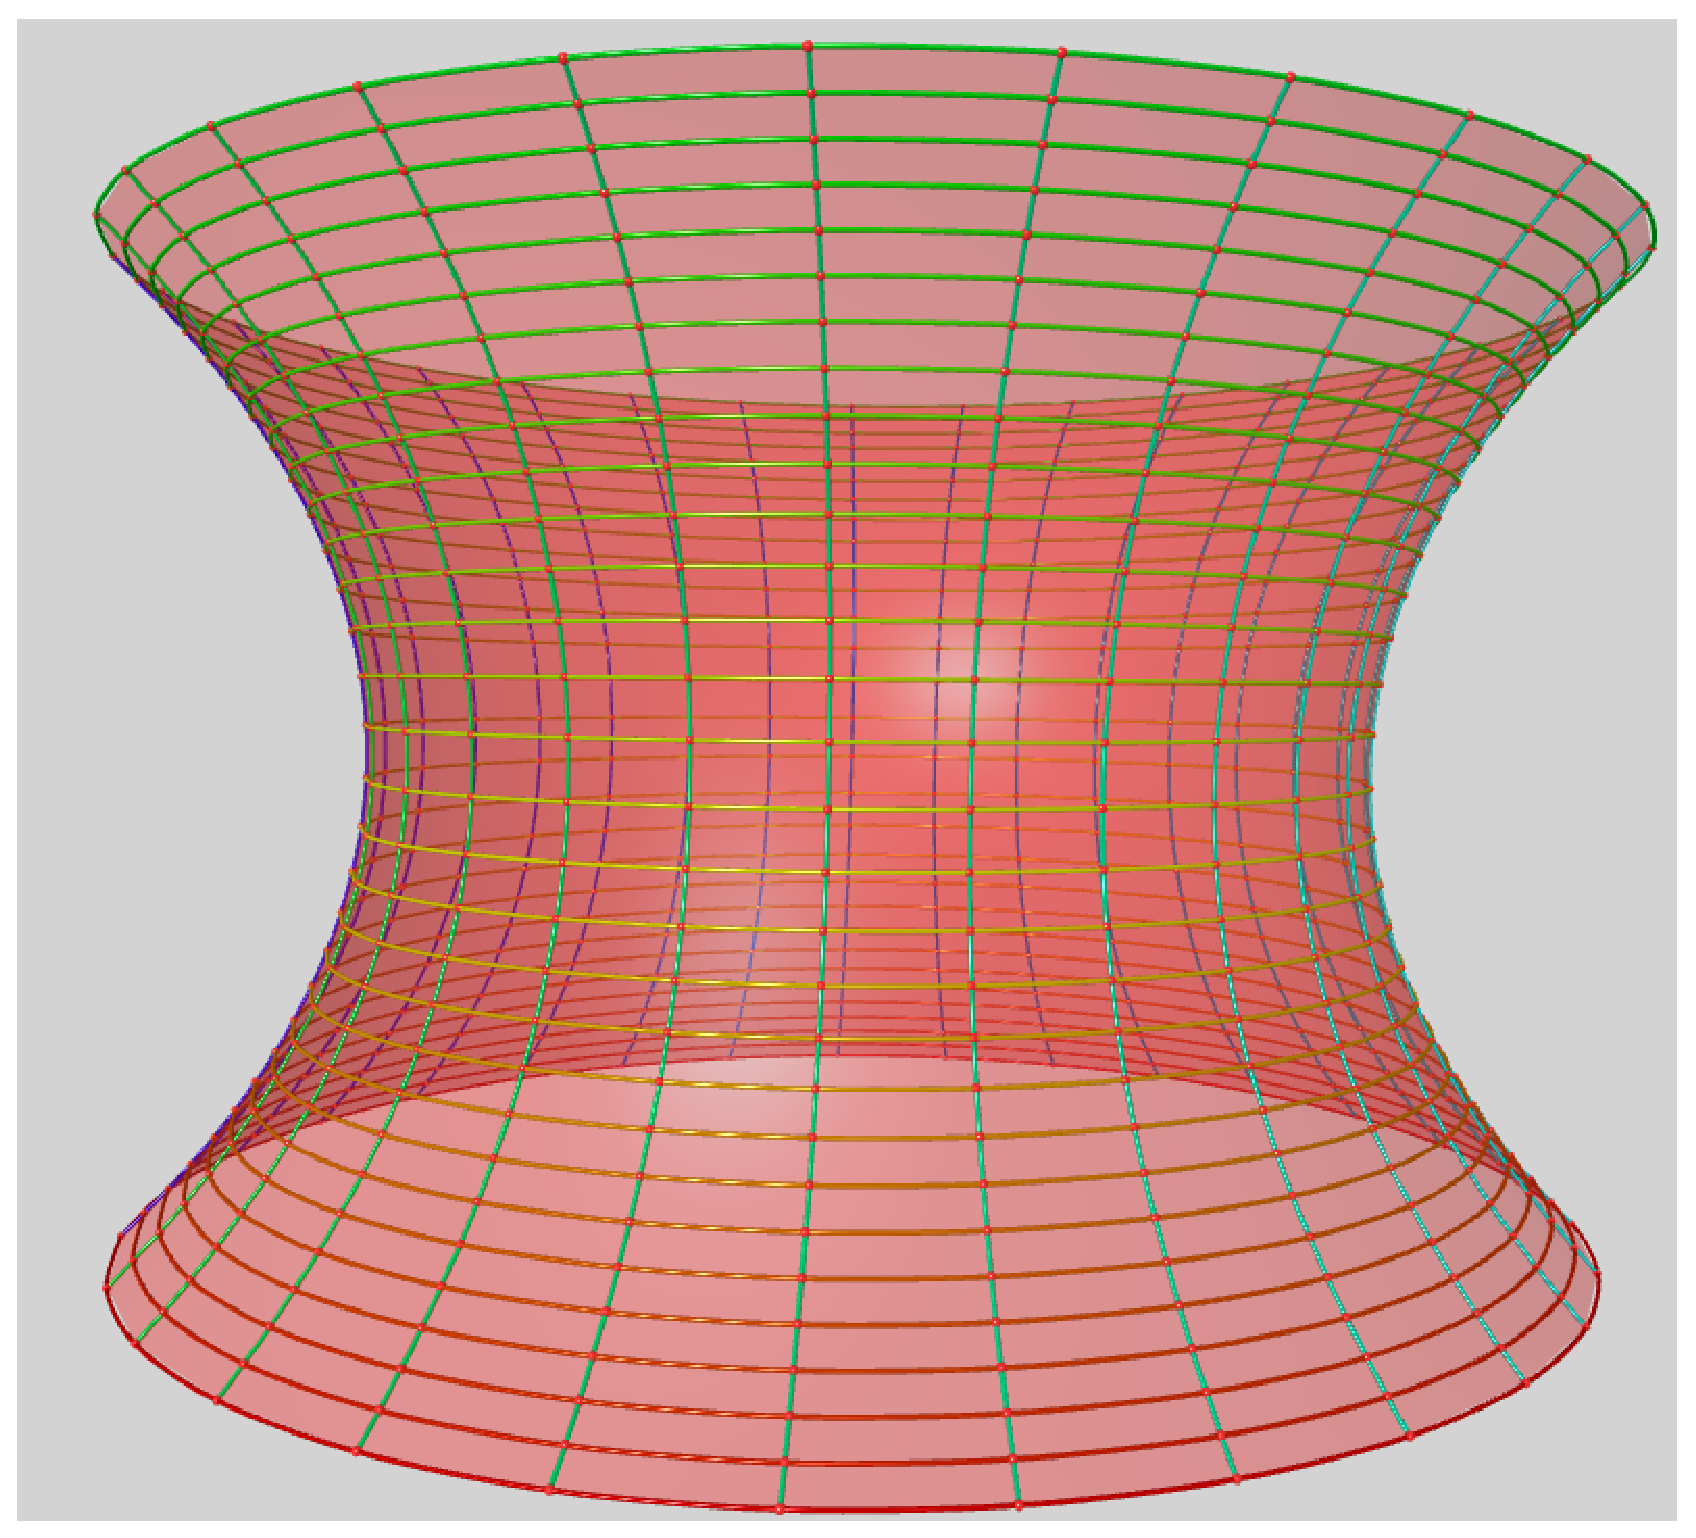
\includegraphics[scale=0.3]{Images_Fichiers/12.eps}
\end{figure}

\subsection[Un hélicoïde]{\uline{Un hélicoïde}}

Pour $G(z)=z$, et $h(z)=\frac{i}{z}$, on obtient l'hélicoïde : 

\begin{figure}[h!]
      \centering 
      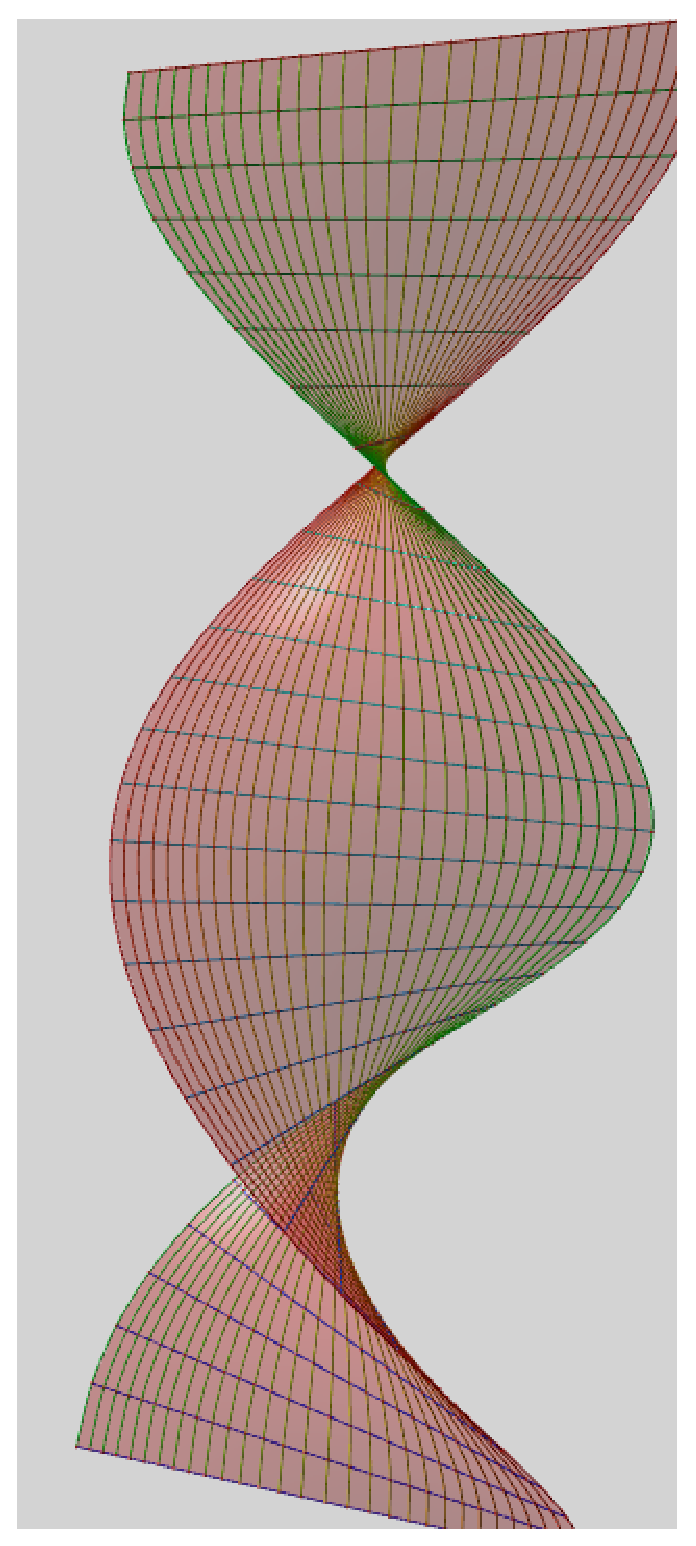
\includegraphics[scale=0.3]{Images_Fichiers/13.eps}
\end{figure}

Arrêtons-nous un instant sur ces deux résultats. Nous voyons que les deux fonctions $h$ des exemples précédents ne diffèrent que d'un facteur $i$. Ces deux surfaces sont donc dites \uline{conjuguées}, et dans ce cas il existe une famille de surfaces minimales permettant de déformer une surface en l'autre, comme nous avons fait dans la première partie de ce rapport avec le caténoïde et l'hélicoïde. 

En effet, pour une surface minimale $\mathscr{M}$ donnée par $G$ et $h$, il suffit de garder le même $G$ et de poser $h_t(z)=e^{t\frac{\pi}{2}}h(z)$ pour avoir une surface minimale pour tout $t\in[0,1]$, la surface $\mathscr{M}$ pour $t=0$, et la surface conjuguée pour $t=1$.

\subsection[La surface d'Enneper]{\uline{La surface d'Enneper}}


Pour $G(z)=z$, et $h(z)=z$, on obtient la surface d'Enneper : 

\begin{figure}[h!]
      \centering 
      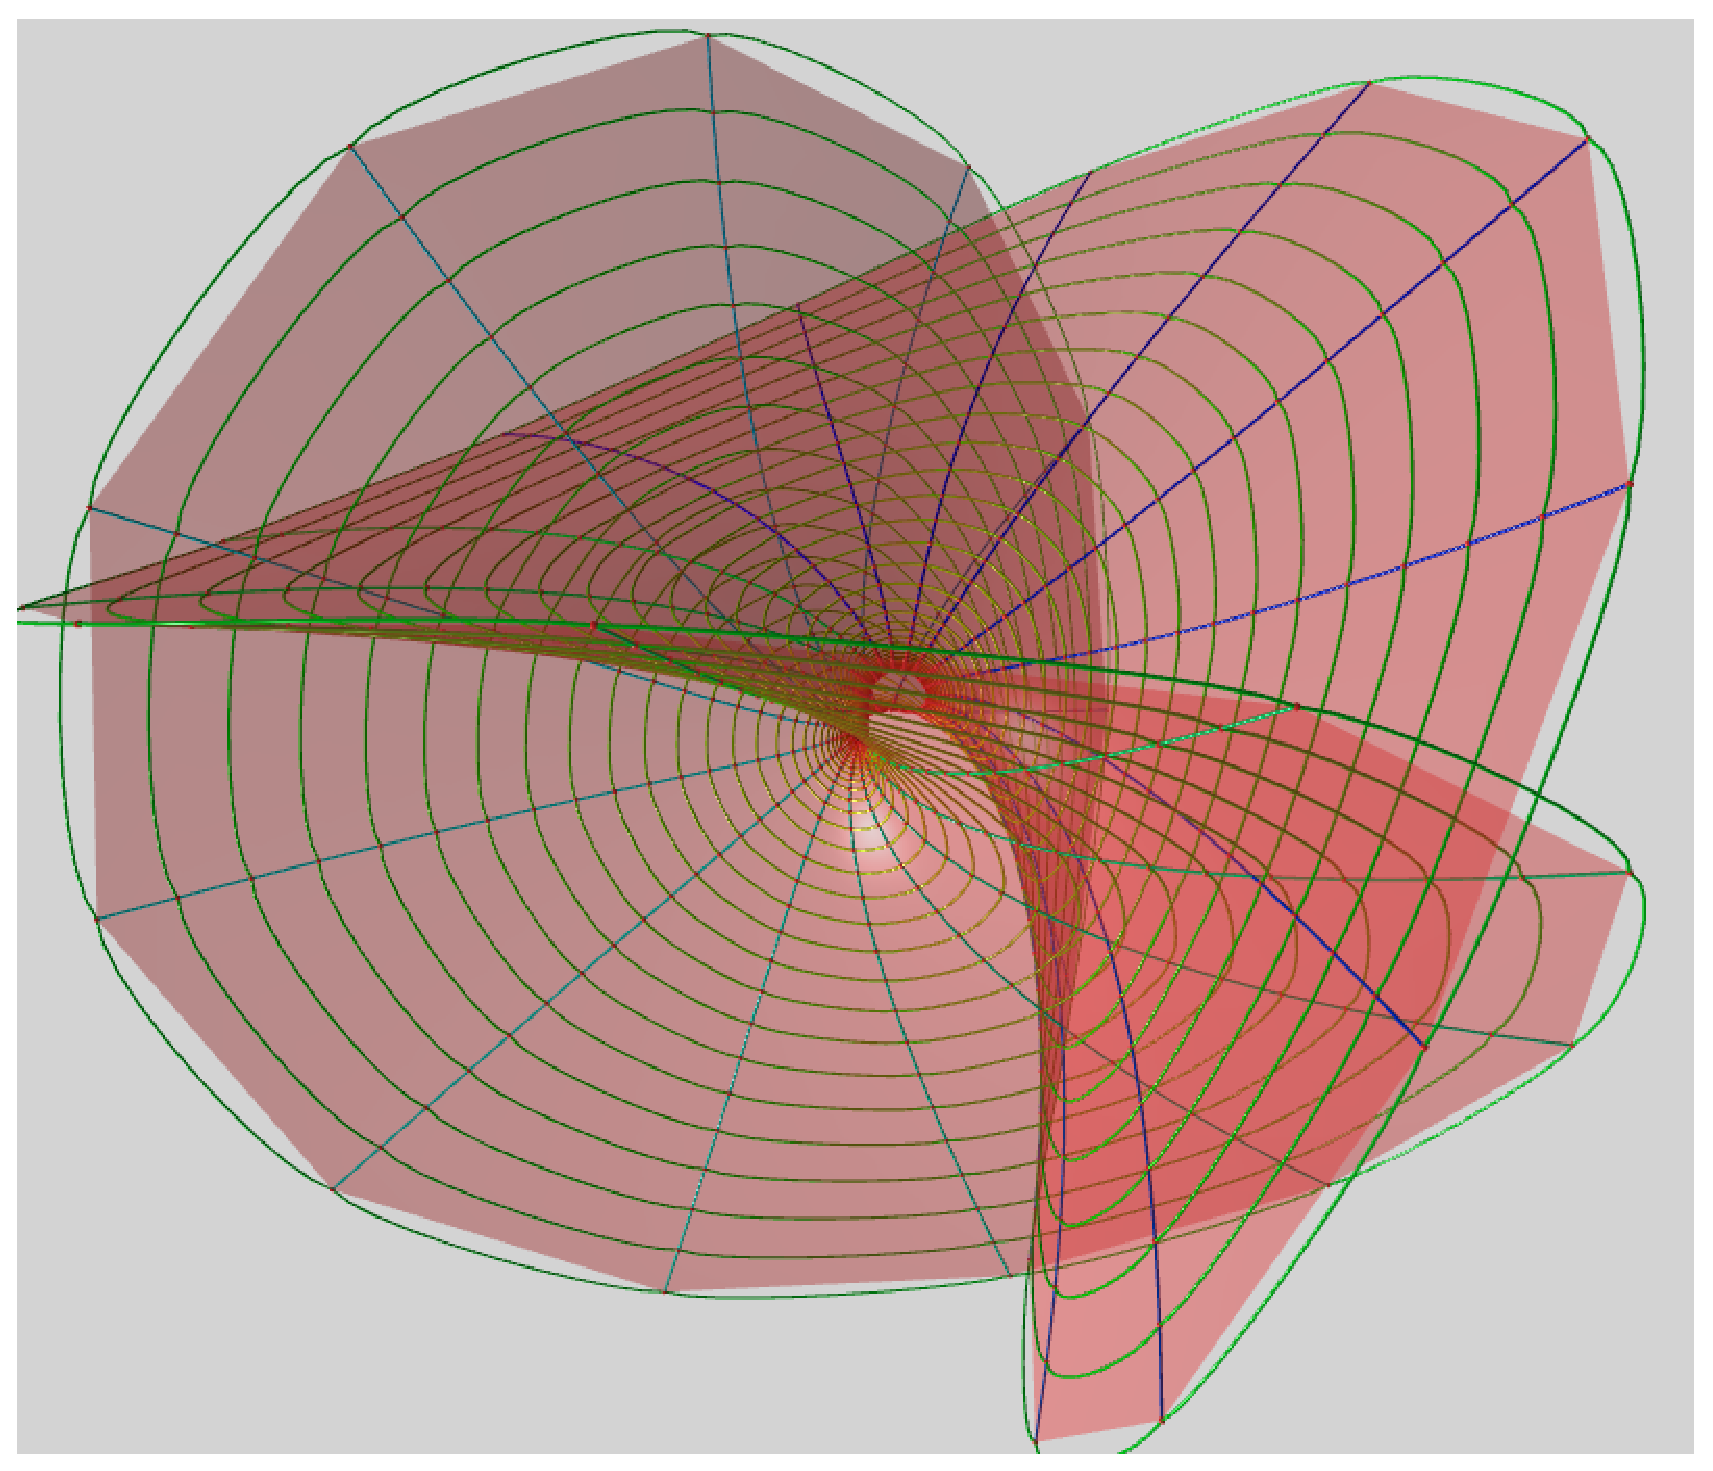
\includegraphics[scale=0.25]{Images_Fichiers/14.eps}
\end{figure}

C'est une surface qui est conjuguée à elle-même et qui possède s'intersecte elle-même. On peut la voir comme une surface minimale dont les bords seraient sur les lignes blanches d'une balle de tennis (approximativement).

\subsection[La fleur de Jenner]{\uline{La fleur de Jenner}}


Pour $G(z)=z$, et $h(z)=z^3$, on obtient la fleur de Jenner : 

\begin{figure}[h!]
      \centering 
      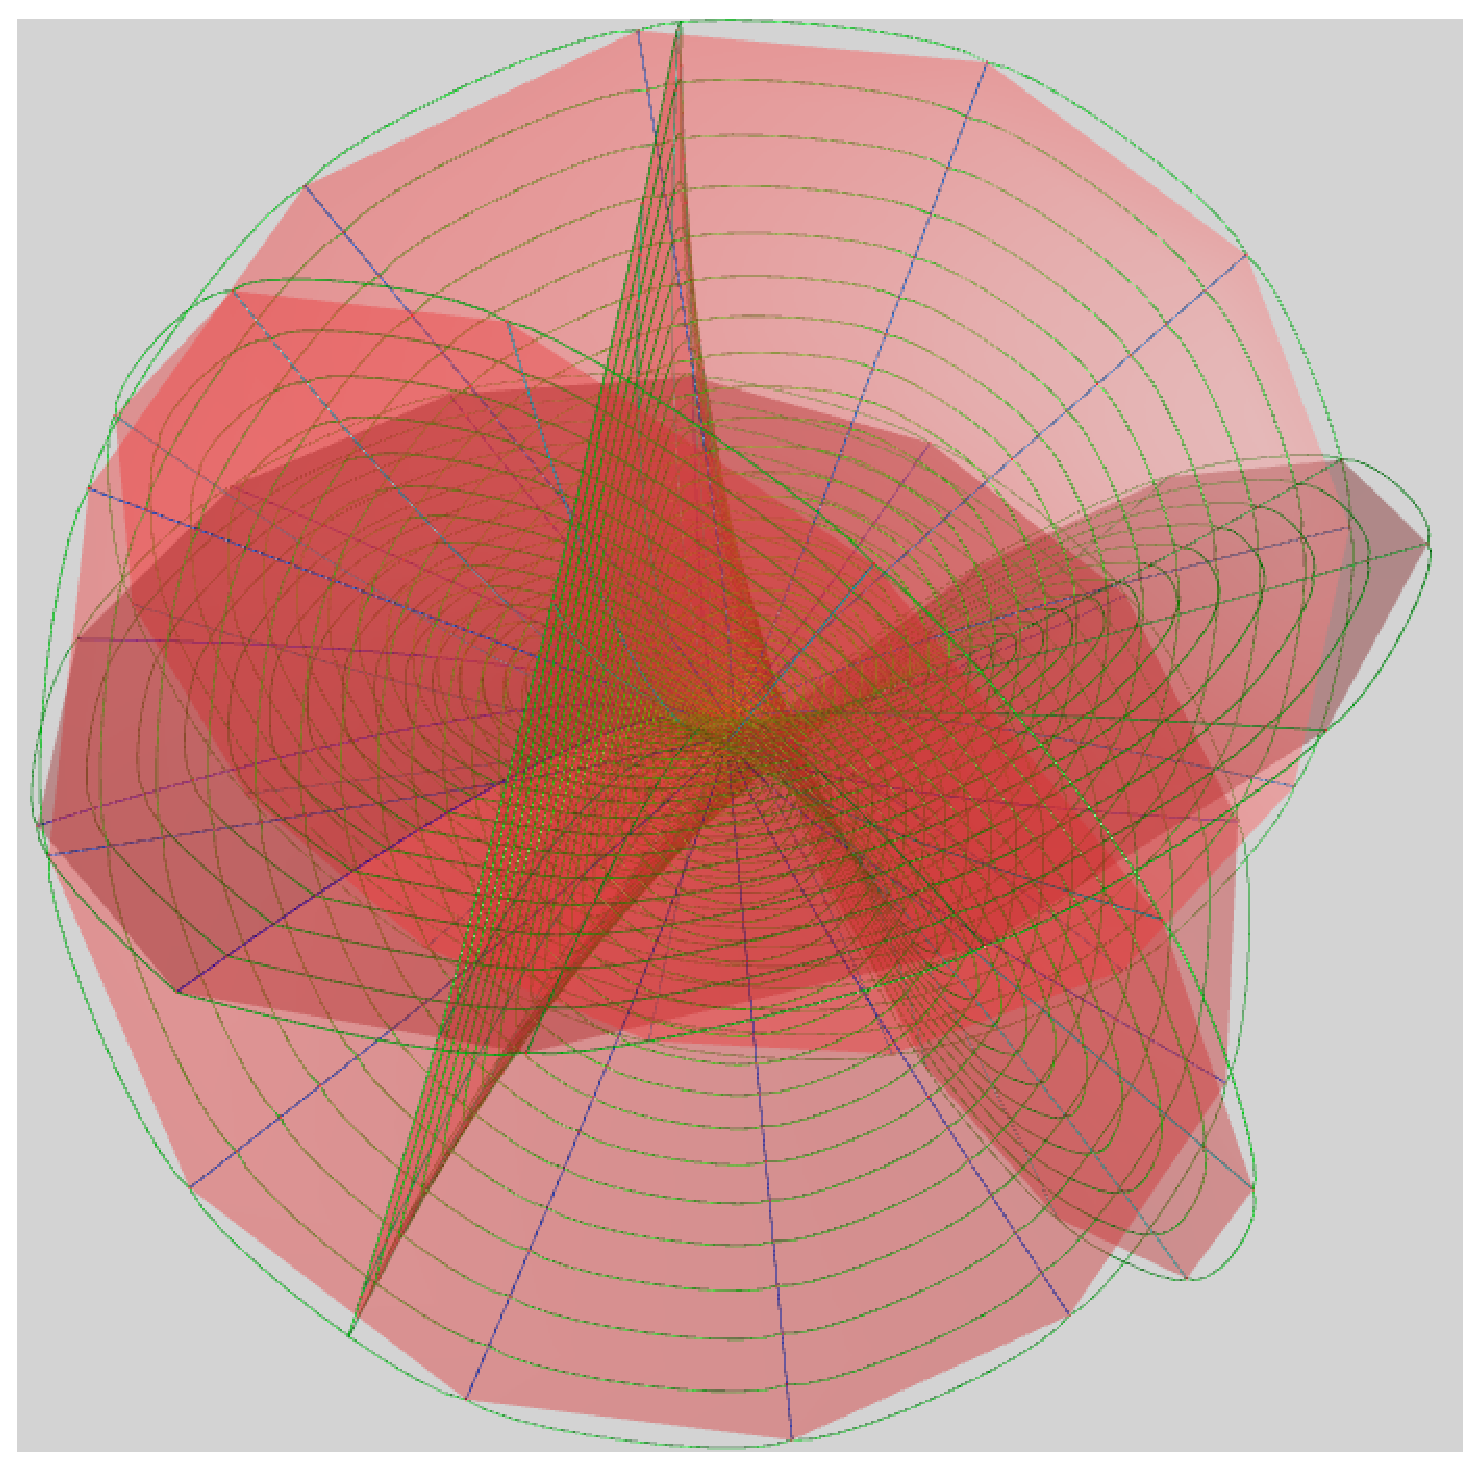
\includegraphics[scale=0.25]{Images_Fichiers/15.eps}
\end{figure}



\chapter[Impressions sur le stage]{\uline{Impressions sur le stage}}

Mon stage de deux mois a débuté assez chaotiquement, étant en même temps très pris par ma profession, les surveillances du bac et mon prochain départ pour l'étranger l'année prochaine. Néanmoins, une fois ces premières semaines passées, j'ai pu me retrouver ensuite avec d'autres étudiants à me consacrer uniquement à cela, et cela s'est avéré passionnant. 

M. Vigon m'avait demandé il y a plusieurs mois si je voulais travailler avec lui et m'a laissé choisir un sujet parmi plusieurs proposés. J'ai choisi celui-ci sans trop de conviction au début, un peu au hasard, surtout parce qu'il y avait de jolies sorties graphiques à faire. En me penchant plus sérieusement sur le sujet, j'ai pu approfondir tout un domaine de la géométrie différentielle que je ne connaissais pas ou peu. 

Les articles étudiés, compliqués à première vue, n'ont finalement pas été aussi difficiles que je l'imaginais à implémenter, la difficulté principale pour moi étant de maîtriser un langage que je ne connaissais pas (Typescript) et la bibliothèque Mathis. Il m'a fallu un peu de temps pour me sentir relativement à l'aise avec ces outils, mais une fois ceci fait, ce fut un véritable plaisir de transcrire les formules des articles en algorithme, et surtout de les voir fonctionner. Ma femme se souvient encore de mon cri de joie quand mon cylindre s'est enfin déformé en caténoïde (ce qui a été compliqué à justifier).

Pour finir, je voudrais chaleureusement remercier M. Vigon pour sa disponibilité pendant ces deux mois, à la fac, par mail et par téléphone, sa sympathie, sa compréhension, et ses explications, toujours limpides ! Ce fut un plaisir pour moi de travailler ensemble.\\
Je remercie également Gwenaël pour le temps qu'il a passé sur son stage (ou sa sieste ??) afin de m'expliquer différents points obscurs pour moi sur Typescript et Mathis. 


\bibliographystyle{abbrv}
\nocite{*}


\bibliography{biblio}



\end{document}
